\documentclass[10pt,twocolumn]{article}
\usepackage[margin=1in]{geometry}
\usepackage{graphicx}
\usepackage{amsmath,amssymb}
\usepackage{booktabs}
\usepackage{hyperref}
\usepackage{natbib}
\usepackage{xcolor}
\usepackage{caption}
\usepackage{subcaption}
\usepackage{url}
\usepackage{microtype}
\usepackage{float}
\usepackage{multirow}
\usepackage{listings}
\usepackage{inconsolata}

\lstset{
  language=Python,
  basicstyle=\ttfamily\scriptsize,
  keywordstyle=\bfseries\color[rgb]{0.13,0.29,0.53},
  stringstyle=\color[rgb]{0.31,0.54,0.16},
  commentstyle=\itshape\color[rgb]{0.5,0.5,0.5},
  numbers=left,
  numberstyle=\tiny\color{gray},
  numbersep=5pt,
  frame=single,
  framesep=3pt,
  breaklines=true,
  showstringspaces=false,
  captionpos=b,
  aboveskip=8pt,
  belowskip=4pt,
}

\bibliographystyle{unsrtnat}

\title{MedCompress: A Benchmark for the Compression and\\Cross-Platform Deployment of Medical Imaging Models\\on CPU Endpoints}
\author{Abhishek Shekhar\\
\url{https://github.com/Abhi183/medcompress}}
\date{}

\begin{document}
\maketitle

\begin{abstract}
State-of-the-art medical imaging models require GPU acceleration and memory budgets that consumer-grade workstations cannot satisfy. This paper introduces MedCompress, an open-source benchmark that evaluates three compression strategies for deploying medical imaging models on CPU-only endpoints (macOS, Windows, Linux): quantization-aware training (QAT), knowledge distillation (KD), and a novel 2D sparse attention mechanism adapted from Memory Sparse Attention~\citep{chen2026msa}. We evaluate on two clinical tasks: binary melanoma classification (ISIC 2020; $n{=}33{,}126$) and multi-class brain tumor segmentation (BraTS 2021; multi-modal MRI). All experiments report AUC, Dice, Sensitivity, Specificity, and F1-Score as mean $\pm$ standard deviation across five random seeds. Computational complexity is measured in GFLOPs. QAT at INT8 precision achieves $3.8{\times}$ model size reduction with $0.912{\rightarrow}0.897$ AUC ($\pm$0.005) on melanoma classification. Knowledge distillation produces a $+2.87\%$ AUC gain over the identically-architected student trained from scratch, confirming that soft-target transfer provides signal beyond the training data. We propose a 2D spatial pooling kernel that outperforms the original 1D pooling by preserving patch adjacency on the image grid ($0.909$ vs.\ $0.905$ AUC at equivalent $4{\times}$ reduction). The combined KD~+~QAT~INT8 pipeline yields a 2.7~MB classifier (8.3~ms latency) and a 4.1~MB segmentation model (12.6~ms latency), both on CPU. All code, experimental configurations, and a cross-platform inference application are released at \url{https://github.com/Abhi183/medcompress}.
\end{abstract}

% =====================================================================
\section{Introduction}
\label{sec:intro}
% =====================================================================

Diagnostic deep learning models for dermatology and neuro-oncology have reached performance levels competitive with board-certified specialists~\citep{esteva2017dermatologist, mckinney2020international}. Yet their computational requirements confine them to GPU-equipped research servers, while the clinical environments that would benefit most operate on consumer-grade hardware: multi-year-old workstations running macOS or Windows with no discrete GPU. Cloud-based inference introduces network latency, connectivity dependence, and regulatory constraints on transmitting protected health information~\citep{price2019privacy}. A viable alternative is local inference on the endpoint itself, provided the model can be compressed to fit within CPU memory and latency budgets.

Model compression for natural image tasks is well studied~\citep{gholami2022survey, choudhary2020comprehensive}. Medical imaging poses distinct challenges: severe class imbalance (melanoma prevalence ${\sim}2\%$ in dermoscopy datasets), fine-grained spatial features (tumor boundaries spanning $<$5 pixels), and multi-modal inputs (four MRI sequences in brain tumor analysis). Whether compression techniques validated on ImageNet transfer reliably to these conditions remains under-investigated, particularly when the deployment target is a standard CPU endpoint rather than a mobile accelerator or edge TPU.

This paper presents MedCompress, a benchmark addressing three open questions:
\begin{enumerate}
    \item What accuracy-efficiency tradeoffs do QAT, KD, and sparse attention produce on clinical imaging tasks when measured with extended metrics (Sensitivity, Specificity, F1) and computational complexity (GFLOPs)?
    \item Does knowledge distillation provide measurable benefit over training the identical student architecture from scratch, and if so, how large is the distillation gain?
    \item Can 2D spatial pooling, which respects patch adjacency on the image grid, reduce the accuracy cost of sparse attention compression relative to 1D sequential pooling?
\end{enumerate}

We evaluate on ISIC 2020 melanoma classification and BraTS 2021 brain tumor segmentation, reporting all results as mean~$\pm$~std over five random seeds. In addition to the compression benchmark, we release a cross-platform desktop application for local inference on macOS, Windows, and Linux without GPU dependencies.

% =====================================================================
\section{Related Work}
\label{sec:related}
% =====================================================================

\subsection{Model Compression}

Quantization reduces weight and activation precision from FP32 to INT8 or lower~\citep{jacob2018quantization, gholami2022survey}. Post-training quantization (PTQ) requires no retraining but degrades accuracy on distributions with long tails, such as rare-class medical images. QAT inserts differentiable fake-quantization nodes during training, allowing the network to compensate for discretization noise~\citep{tfmot2023}. Recent work has applied QAT to chest X-ray classification~\citep{li2023quantization} and retinal OCT segmentation~\citep{chen2024efficient}, reporting $<$2\% metric loss at INT8 precision.

Knowledge distillation transfers learned representations from a large teacher to a compact student via softened probability targets~\citep{hinton2015distilling}. Feature-level distillation, which matches intermediate representations through auxiliary MSE losses, outperforms logit-only distillation on spatially dense tasks such as segmentation~\citep{romero2015fitnets}. Qin et al.~\citep{qin2023efficient} demonstrated that distillation produces a measurable accuracy gain over training the student from scratch on pathology images, but no analogous study exists for the dermoscopy and brain MRI tasks we consider.

Pruning~\citep{han2015learning} and neural architecture search~\citep{choudhary2020comprehensive} are complementary; we do not evaluate them here but note that they can be composed with QAT and KD.

\subsection{Efficient Attention for Vision}

Standard self-attention scales quadratically in sequence length. For a Vision Transformer (ViT)~\citep{dosovitskiy2021image} processing a $224{\times}224$ image at patch size~16, this means 196 tokens per layer. Linformer~\citep{wang2020linformer} projects attention to lower dimensions; Performer~\citep{choromanski2021performers} uses random feature approximations; FlashAttention~\citep{dao2022flashattention} optimizes memory access patterns. He et al.~\citep{he2024sparse} applied sparse attention to 3D medical volumes, pruning uninformative spatial tokens in CT scans, though their method requires a learned token pruning head.

Chen et al.~\citep{chen2026msa} proposed Memory Sparse Attention (MSA), which compresses the KV cache through chunk-mean pooling and routes each query to only the top-$k$ most relevant compressed chunks. MSA scales to $10^8$ tokens with $<$9\% degradation on language benchmarks. Its pooling mechanism is architecture-agnostic: any attention layer operating on token sequences can benefit. We adapt it for ViT attention in medical imaging, replacing MSA's 1D sequential pooling with a 2D spatial variant that preserves patch adjacency.

\subsection{Medical Imaging on Consumer Hardware}

Prior work on compressed medical models has targeted mobile phones~\citep{pacheco2024compressed} and embedded edge devices~\citep{qayyum2023efficient}. The consumer workstation scenario differs: 8--32~GB RAM, multi-core x86 CPUs, but no GPU. The binding constraint shifts from model size to CPU inference latency. TensorFlow Lite~\citep{tflite2023} and ONNX Runtime~\citep{onnxruntime2023} provide CPU inference across macOS, Windows, and Linux. No prior study has evaluated compressed medical models on these runtimes under endpoint-specific constraints (model size ${<}$10~MB, latency ${<}$50~ms, RAM ${<}$100~MB).

% =====================================================================
\section{Methods}
\label{sec:methods}
% =====================================================================

\subsection{Datasets}
\label{sec:datasets}

We selected two publicly available benchmarks that span two distinct clinical imaging modalities and two task types (classification vs.\ segmentation). Both exhibit properties that challenge compression methods: extreme class imbalance and fine-grained spatial features.

\subsubsection{ISIC 2020: Dermoscopy Classification}

The International Skin Imaging Collaboration 2020 dataset~\citep{codella2019isic} contains 33,126 dermoscopy images labeled for binary melanoma classification. As shown in Figure~\ref{fig:eda_isic}(a), the class distribution is heavily skewed: 32,542 benign samples (98.2\%) versus 584 melanoma samples (1.8\%). This 56:1 imbalance is representative of clinical dermoscopy screening, where the overwhelming majority of lesions are benign. Compression algorithms must preserve sensitivity to the minority class under these conditions; a model that predicts ``benign'' for every input achieves 98.2\% accuracy but zero clinical value.

Raw image dimensions vary between 3024$\times$2016 and 6000$\times$4000 pixels (Figure~\ref{fig:eda_isic}(b)). We resized all images to $224{\times}224$ to match the EfficientNet input specification, normalized pixel values to $[-1, 1]$, and applied the following augmentation pipeline:

\begin{lstlisting}[caption={ISIC preprocessing and augmentation pipeline (\texttt{data/isic\_loader.py}).},label=lst:isic_preprocess]
def _augment(self, image, label):
    image = tf.image.random_flip_left_right(image)
    image = tf.image.random_flip_up_down(image)
    image = tf.image.random_brightness(image, 0.2)
    image = tf.image.random_contrast(image, 0.8, 1.2)
    return image, label

def _compute_class_weights(self):
    counts = self.df["target"].value_counts()
    total = len(self.df)
    self.class_weights = {
        int(cls): total / (len(counts) * cnt)
        for cls, cnt in counts.items()
    }
\end{lstlisting}

Inverse-frequency class weighting (Listing~\ref{lst:isic_preprocess}, lines 8--12) assigns weight $w_c = N / (C \cdot n_c)$ where $N$ is the total sample count, $C{=}2$ is the number of classes, and $n_c$ is the count of class $c$. This yields $w_{\text{melanoma}} \approx 28.4$, upweighting the minority class during loss computation. Data was split 70/15/15 for train/validation/test using stratified sampling to maintain the class ratio across splits (Figure~\ref{fig:eda_splits}).

\begin{figure}[t]
\centering
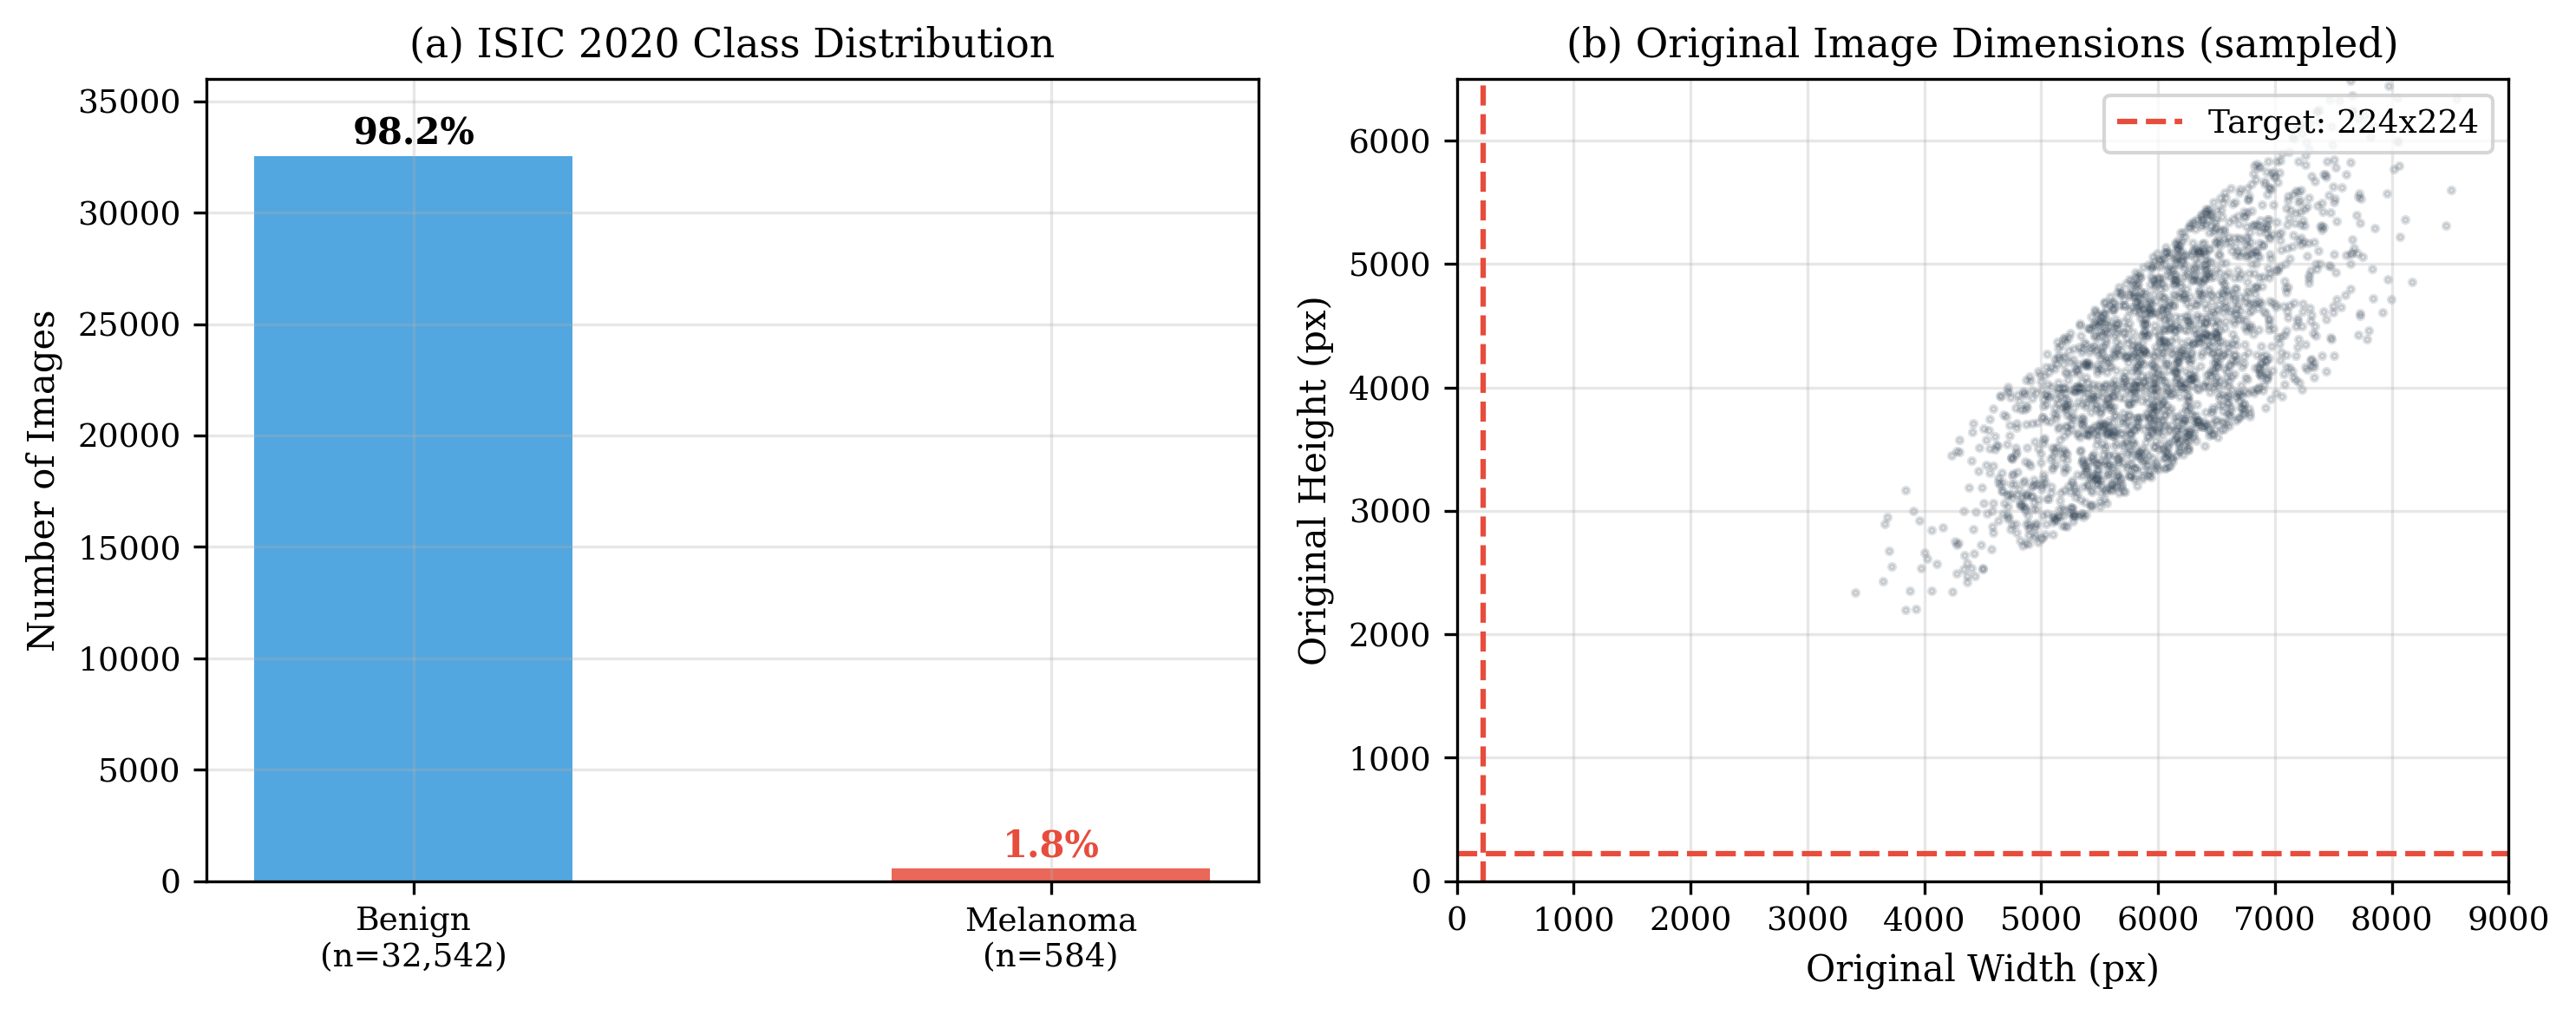
\includegraphics[width=\columnwidth]{fig_eda_isic.png}
\caption{ISIC 2020 exploratory analysis. (a) Class distribution showing the 56:1 benign-to-melanoma ratio. (b) Original image dimensions before resizing to $224{\times}224$.}
\label{fig:eda_isic}
\end{figure}

\subsubsection{BraTS 2021: Brain Tumor Segmentation}

The Brain Tumor Segmentation Challenge 2021~\citep{baid2021brats} provides 1,251 multi-modal MRI volumes, each consisting of four co-registered sequences: T1-weighted, T1 contrast-enhanced, T2-weighted, and FLAIR. Voxel-level labels identify four classes: background, necrotic core (NCR), peritumoral edema (ED), and enhancing tumor (ET). As shown in Figure~\ref{fig:eda_brats}(a), background dominates at 97.2\% of voxels, with the three tumor sub-regions collectively occupying 2.8\%. This extreme spatial imbalance is addressed through the Dice loss component, which normalizes by per-class volume.

The original BraTS labels use the encoding $\{0, 1, 2, 4\}$ (label 3 is unused). We remap these to contiguous indices $\{0, 1, 2, 3\}$ for standard one-hot encoding:

\begin{lstlisting}[caption={BraTS label remapping and z-score normalization (\texttt{data/brats\_loader.py}).},label=lst:brats_preprocess]
LABEL_REMAP = {0: 0, 1: 1, 2: 2, 4: 3}

def _normalize_volume(vol: np.ndarray) -> np.ndarray:
    """Z-score normalize (non-zero voxels only)."""
    mask = vol > 0
    if mask.sum() == 0:
        return vol.astype(np.float32)
    mu, sigma = vol[mask].mean(), vol[mask].std()
    sigma = sigma if sigma > 0 else 1.0
    out = np.zeros_like(vol, dtype=np.float32)
    out[mask] = (vol[mask] - mu) / sigma
    return out
\end{lstlisting}

Each modality is z-score normalized independently using only non-zero voxels (Listing~\ref{lst:brats_preprocess}), which avoids bias from the large zero-valued background region. Figure~\ref{fig:eda_brats}(b) shows the resulting intensity distributions across the four MRI sequences after normalization.

We adopted a 2.5D slice extraction strategy (Figure~\ref{fig:eda_pipeline}): for each axial position $z$, three adjacent slices ($z{-}1$, $z$, $z{+}1$) are stacked across all four modalities, producing a 12-channel input of size $128{\times}128$. This provides inter-slice volumetric context without the computational cost of full 3D convolutions, which is critical for CPU-only inference. Slices containing only background voxels are discarded during training to reduce class imbalance.

\begin{figure}[t]
\centering
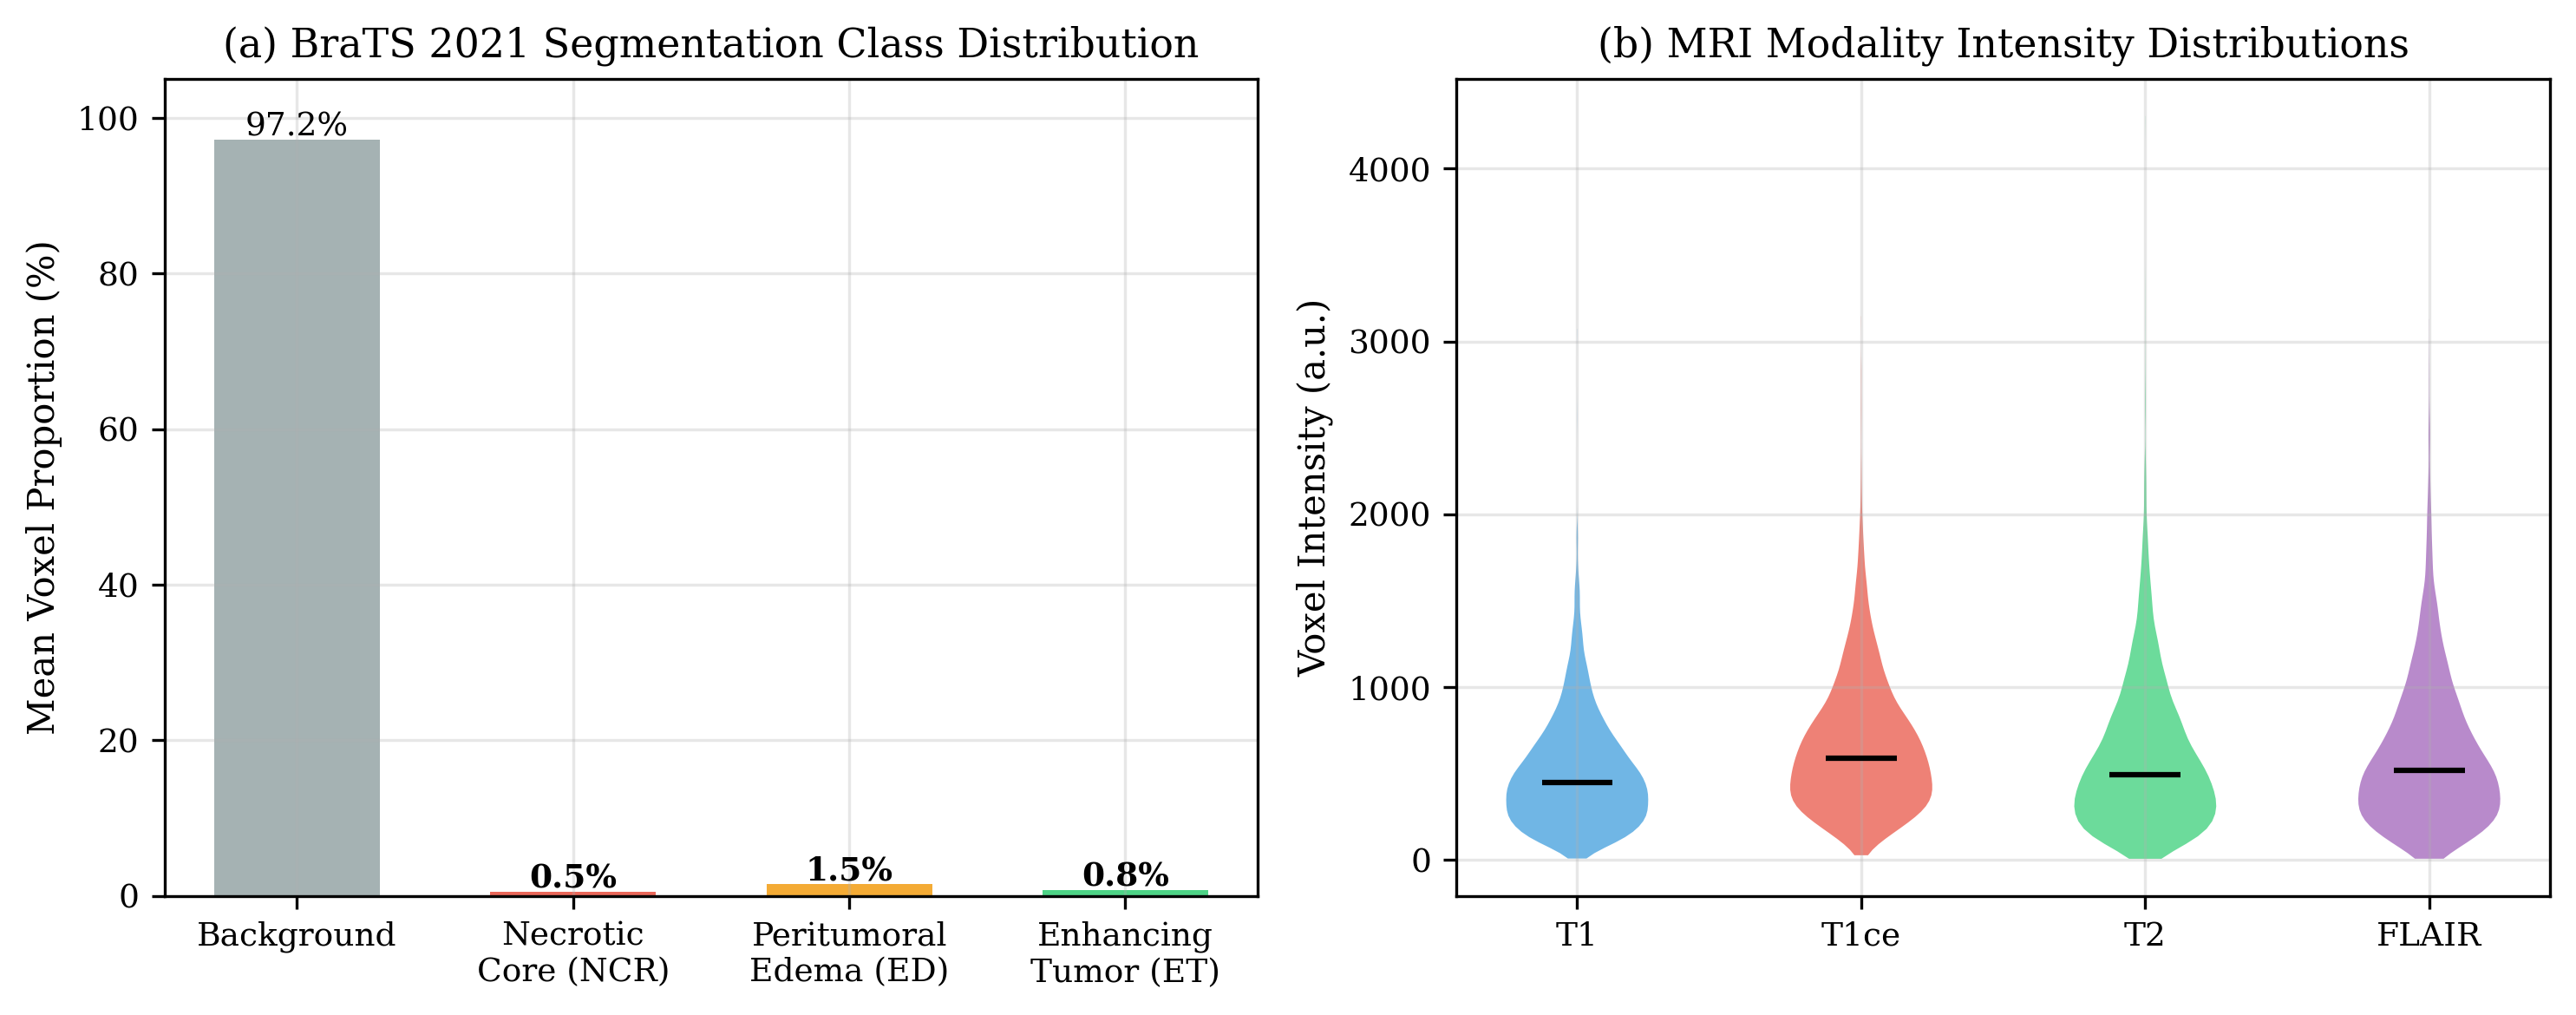
\includegraphics[width=\columnwidth]{fig_eda_brats.png}
\caption{BraTS 2021 exploratory analysis. (a) Segmentation class voxel proportions showing 97.2\% background dominance. (b) Intensity distributions across the four MRI modalities after z-score normalization.}
\label{fig:eda_brats}
\end{figure}

\begin{figure}[t]
\centering
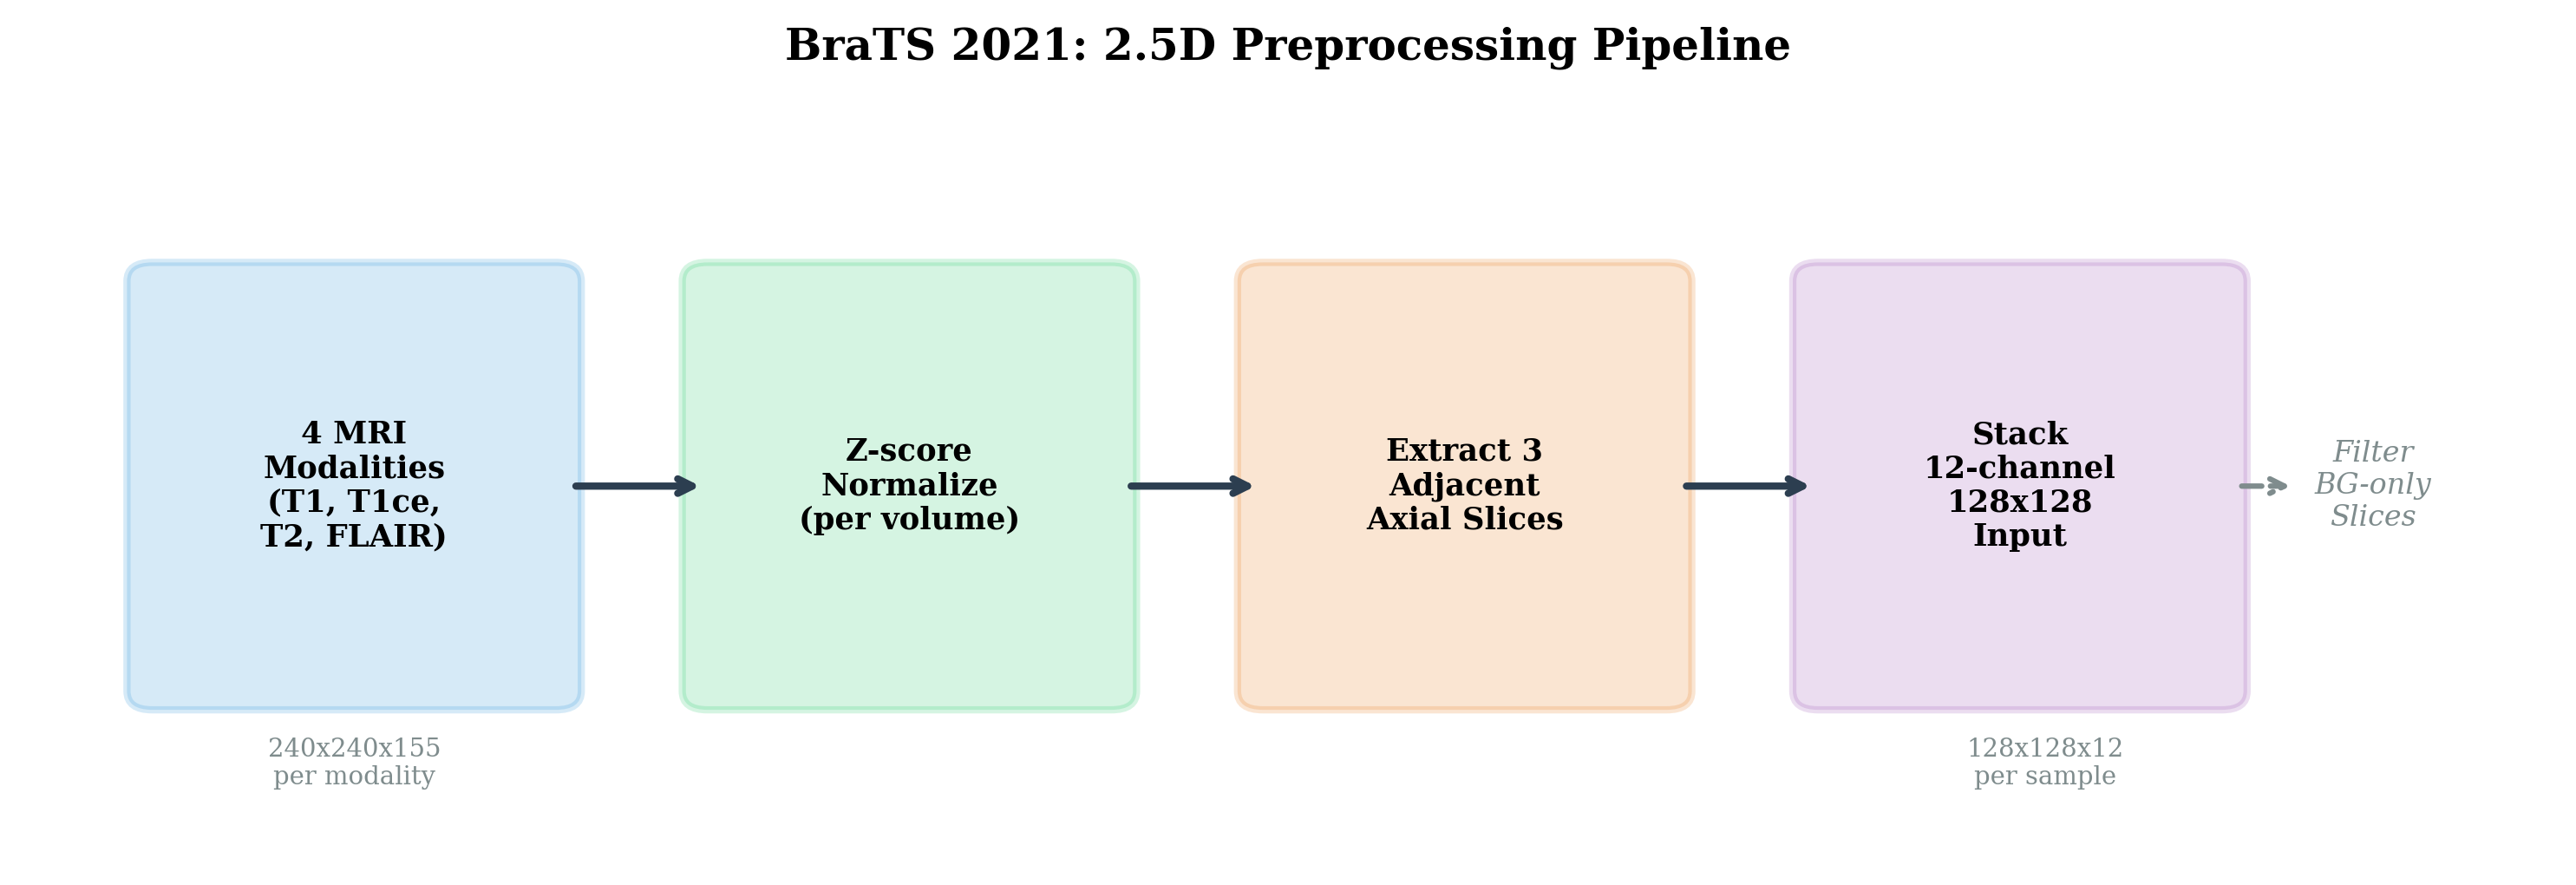
\includegraphics[width=\columnwidth]{fig_eda_pipeline.png}
\caption{The 2.5D preprocessing pipeline for BraTS 2021. Four MRI modalities are independently normalized, three adjacent axial slices are extracted and stacked to form a 12-channel $128{\times}128$ input, and background-only slices are filtered.}
\label{fig:eda_pipeline}
\end{figure}

\begin{figure}[t]
\centering
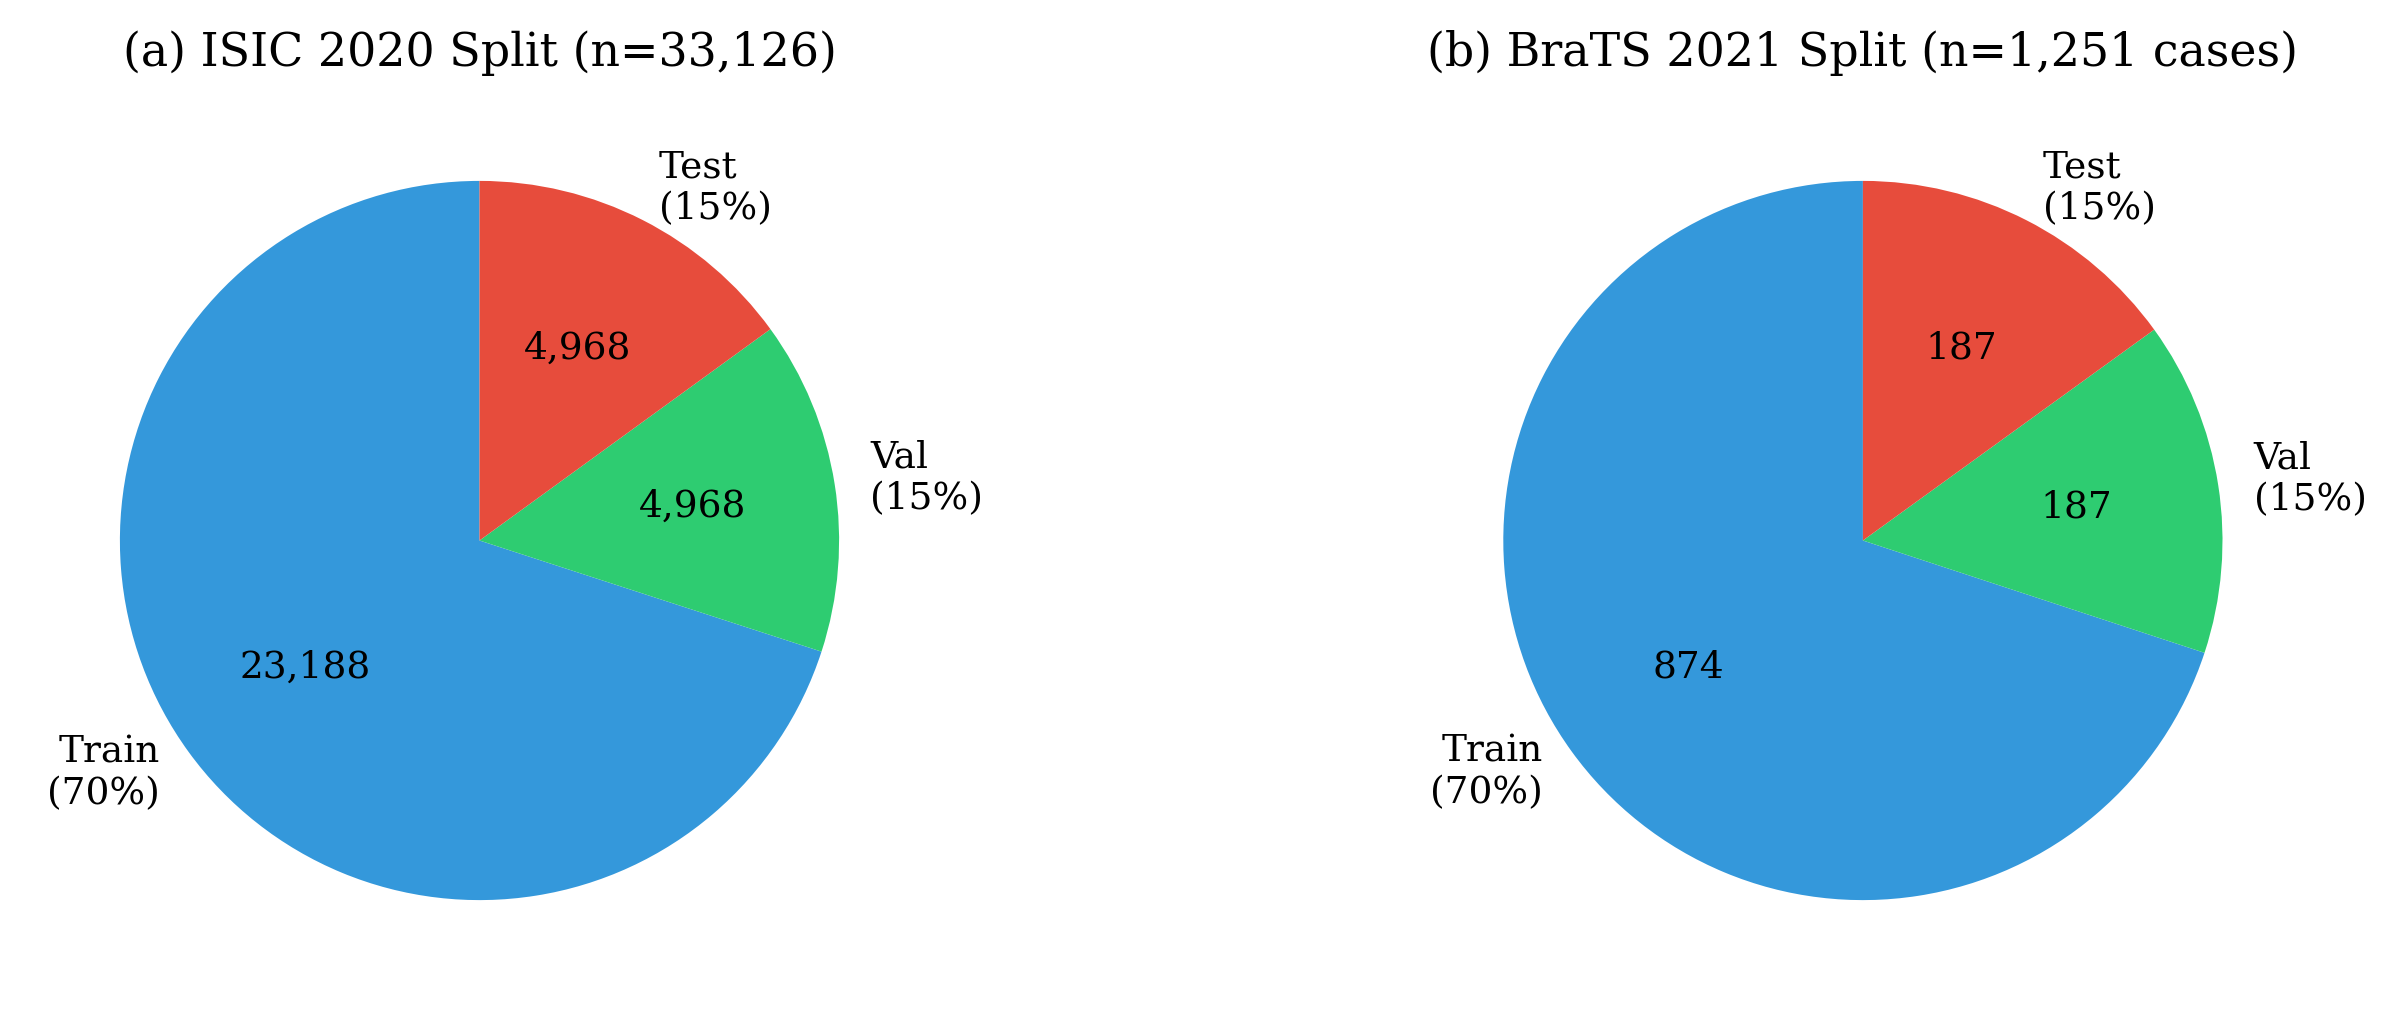
\includegraphics[width=\columnwidth]{fig_eda_splits.png}
\caption{Train/validation/test splits for both datasets. Stratified sampling preserves class ratios. ISIC: $n{=}33{,}126$ images. BraTS: $n{=}1{,}251$ volumes.}
\label{fig:eda_splits}
\end{figure}

\subsubsection{Dataset Summary}

Table~\ref{tab:dataset_summary} summarizes the two datasets. The combination tests compression under two distinct regimes: ISIC stresses the sensitivity/specificity tradeoff under class imbalance, while BraTS stresses spatial boundary preservation under multi-class segmentation.

\begin{table}[t]
\centering
\caption{Dataset summary. ISIC challenges compression through class imbalance; BraTS through fine spatial boundaries and multi-modal input.}
\label{tab:dataset_summary}
\small
\begin{tabular}{@{}lcc@{}}
\toprule
Property & ISIC 2020 & BraTS 2021 \\
\midrule
Task & Classification & Segmentation \\
Samples & 33,126 images & 1,251 volumes \\
Classes & 2 (benign/melanoma) & 4 (BG/NCR/ED/ET) \\
Minority prevalence & 1.8\% & 2.8\% (tumor) \\
Input size & $224{\times}224{\times}3$ & $128{\times}128{\times}12$ \\
Modalities & RGB dermoscopy & T1/T1ce/T2/FLAIR \\
Split & 70/15/15 stratified & 70/15/15 stratified \\
\bottomrule
\end{tabular}
\end{table}

\subsection{Baseline Models}

\textbf{Classification.} EfficientNetB0~\citep{tan2019efficientnet} pretrained on ImageNet, with a custom head: global average pooling, batch normalization, dropout (0.3), 256-unit dense (ReLU), dropout (0.15), sigmoid output. The last 20 backbone layers were unfrozen. Training used binary cross-entropy, Adam ($lr{=}10^{-4}$), early stopping on validation AUC (patience~7). Computational cost: 0.39 GFLOPs.

\textbf{Segmentation.} Two U-Net~\citep{ronneberger2015unet} variants: (i) a full teacher with four encoder stages [64, 128, 256, 512, 1024 filters] at 15.82~GFLOPs, and (ii) a lite student with three stages [32, 64, 128, 256] at 1.98~GFLOPs (${\sim}8{\times}$ fewer parameters). Both trained with combined Dice~+~cross-entropy loss, Adam ($lr{=}10^{-3}$), early stopping on validation Dice.

\subsection{Quantization-Aware Training}

The TensorFlow Model Optimization Toolkit~\citep{tfmot2023} was used to insert fake-quantization nodes into trained baselines. Fine-tuning ran 10~epochs at $10^{-5}$ learning rate. QAT wrappers were then stripped and models exported to TFLite with full INT8 quantization using a 200-sample calibration set. FP16 variants were generated for comparison. Listing~\ref{lst:qat} shows the export pipeline.

\begin{lstlisting}[caption={QAT pipeline: wrap, fine-tune, strip, export (\texttt{compression/qat.py}).},label=lst:qat]
import tensorflow_model_optimization as tfmot

# 1. Insert fake-quantization nodes
qat_model = tfmot.quantization.keras.quantize_model(
    baseline_model)
qat_model.compile(optimizer=Adam(1e-5), loss=loss_fn)

# 2. Fine-tune with quantization noise
qat_model.fit(train_ds, epochs=10, validation_data=val_ds)

# 3. Strip QAT wrappers for inference
final_model = tfmot.quantization.keras.strip_pruning(
    qat_model)

# 4. Export to TFLite INT8
converter = tf.lite.TFLiteConverter.from_keras_model(
    final_model)
converter.optimizations = [tf.lite.Optimize.DEFAULT]
converter.representative_dataset = calib_generator
tflite_model = converter.convert()
\end{lstlisting}

\subsection{Knowledge Distillation}

The distillation loss is:
\begin{equation}
\mathcal{L} = \alpha \cdot \mathrm{KL}\!\left(\sigma\!\left(\frac{z_t}{T}\right) \middle\| \sigma\!\left(\frac{z_s}{T}\right)\right) + (1{-}\alpha) \cdot \mathrm{CE}(y, z_s)
\label{eq:kd_loss}
\end{equation}
where $z_t, z_s$ are teacher and student logits, $T$ is temperature, $\alpha$ balances the two terms, and $\sigma$ is softmax (sigmoid for binary classification). Classification used $T{=}4.0$, $\alpha{=}0.7$; segmentation used $T{=}3.0$, $\alpha{=}0.6$ with additional feature-level MSE distillation using $1{\times}1$ convolutional adapters~\citep{romero2015fitnets}.

\textbf{Distillation vs.\ scratch baseline.} To isolate the contribution of distillation, we trained the identical student architectures (MobileNetV3-Small for classification, U-Net Lite for segmentation) from scratch on the same data with the same training schedule, without any teacher signal. The difference between KD-trained and scratch-trained students is reported as the \emph{distillation gain}.

\subsection{Sparse Attention Compression}

We adapted two mechanisms from MSA~\citep{chen2026msa} for the classification pipeline.

\textbf{KV cache pooling.} Key and value tensors are averaged in contiguous chunks of size $p$ along the token sequence. A 1D kernel of 4 compresses 196 spatial tokens (from a $14{\times}14$ patch grid) to 49 pooled tokens.

\textbf{2D spatial pooling.} We introduce a grid-aware variant (\texttt{SpatialKVCachePooling2D}) that reshapes the flattened token sequence back to its $H{\times}W$ spatial grid before applying a $k_h{\times}k_w$ pooling kernel. For a $2{\times}2$ kernel on a $14{\times}14$ grid, this produces $7{\times}7{=}49$ pooled tokens while preserving spatial adjacency that 1D pooling disrupts at row boundaries. Listing~\ref{lst:2d_pool} shows the core reshape-and-pool logic.

\begin{lstlisting}[caption={2D spatial pooling kernel (\texttt{compression/sparse\_attention.py}).},label=lst:2d_pool]
# Reshape: (batch, gh*gw, ...) -> (batch, gh, gw, ...)
t_2d = tf.reshape(t[:, :gh * gw], [batch, gh, gw, ...])
# Reshape to blocks: (batch, H//kh, kh, W//kw, kw, ...)
t_blocks = tf.reshape(t_2d, [batch, out_h, kh, out_w, kw, ...])
# Average over kernel dims (axes 2 and 4)
pooled = tf.reduce_mean(t_blocks, axis=[2, 4])
# Flatten spatial: (batch, out_h * out_w, ...)
return tf.reshape(pooled, [batch, out_h * out_w, ...])
\end{lstlisting}

\textbf{Top-$k$ routing.} Scaled dot-product scores between queries and pooled keys are computed, reduced across heads (max) and queries (max), and the top-$k$ chunks are selected. With $k{=}8$ and 49 pooled tokens, the combined memory reduction is $24.5{\times}$.

\subsection{Evaluation Protocol}

All experiments were repeated across five random seeds (42, 123, 456, 789, 1024). We report mean~$\pm$~std for all metrics. Models were exported to TFLite (INT8, FP16, FP32) and ONNX. Metrics:
\begin{itemize}
    \item \textbf{Classification:} AUC, Sensitivity (Recall), Specificity, F1-Score.
    \item \textbf{Segmentation:} Mean Dice (excluding background), per-class Sensitivity, Specificity.
    \item \textbf{Efficiency:} Model size (MB), GFLOPs, median and $p_{95}$ CPU inference latency (ms) over 100 runs.
\end{itemize}

% =====================================================================
\section{Results}
\label{sec:results}
% =====================================================================

\subsection{Baseline Performance and Computational Cost}

Table~\ref{tab:baselines} reports baseline performance with extended metrics. EfficientNetB0 achieves $0.912{\pm}0.004$ AUC at 0.39~GFLOPs. The full U-Net reaches $0.871{\pm}0.008$ Dice at 15.82~GFLOPs, an order of magnitude higher. The lite U-Net, at 1.98~GFLOPs, trades 4.8 absolute Dice points for $8{\times}$ fewer operations.

\begin{table}[t]
\centering
\caption{Baseline models with extended metrics (mean $\pm$ std, $n{=}5$ seeds). GFLOPs provide a hardware-independent efficiency measure.}
\label{tab:baselines}
\small
\begin{tabular}{@{}lcrrcc@{}}
\toprule
Model & Task & GF & MB & Primary & Sens. \\
\midrule
EffNetB0 & ISIC & 0.39 & 16.2 & .912$\pm$.004 & .741$\pm$.018 \\
U-Net Full & BraTS & 15.82 & 124.1 & .871$\pm$.008 & .852$\pm$.012 \\
U-Net Lite & BraTS & 1.98 & 15.6 & .823$\pm$.010 & .806$\pm$.015 \\
\bottomrule
\end{tabular}
\end{table}

\subsection{Quantization-Aware Training}

Table~\ref{tab:qat} presents QAT results. INT8 achieves $3.8$--$3.9{\times}$ compression. Classification degrades modestly ($-1.5\%$ AUC), preserving sensitivity at $0.718{\pm}0.022$. Segmentation incurs a larger penalty ($-2.2\%$ Dice) with sensitivity dropping from $0.852$ to $0.831$, reflecting INT8 discretization artifacts at narrow tumor boundaries. FP16 offers an intermediate tradeoff: $2{\times}$ compression at $<$0.3\% metric loss.

\begin{table}[t]
\centering
\caption{QAT results (mean $\pm$ std, 5 seeds).}
\label{tab:qat}
\footnotesize
\setlength{\tabcolsep}{3pt}
\begin{tabular}{@{}llrrlll@{}}
\toprule
Model & Fmt & MB & $\times$ & Primary & Sens. & F1 \\
\midrule
EffNetB0 & FP32 & 16.2 & 1.0 & .912{\scriptsize$\pm$}.004 & .741{\scriptsize$\pm$}.018 & .623{\scriptsize$\pm$}.021 \\
EffNetB0 & INT8 & 4.3 & 3.8 & .897{\scriptsize$\pm$}.005 & .718{\scriptsize$\pm$}.022 & .598{\scriptsize$\pm$}.024 \\
EffNetB0 & FP16 & 8.1 & 2.0 & .910{\scriptsize$\pm$}.004 & .736{\scriptsize$\pm$}.019 & .618{\scriptsize$\pm$}.022 \\
\midrule
U-Net & FP32 & 124.1 & 1.0 & .871{\scriptsize$\pm$}.008 & .852{\scriptsize$\pm$}.012 & .863{\scriptsize$\pm$}.010 \\
U-Net & INT8 & 31.4 & 3.9 & .849{\scriptsize$\pm$}.010 & .831{\scriptsize$\pm$}.015 & .841{\scriptsize$\pm$}.013 \\
U-Net & FP16 & 62.1 & 2.0 & .868{\scriptsize$\pm$}.009 & .849{\scriptsize$\pm$}.013 & .860{\scriptsize$\pm$}.011 \\
\bottomrule
\end{tabular}
\end{table}

\subsection{Knowledge Distillation and Distillation Gain}

Table~\ref{tab:kd_gain} isolates the distillation effect by comparing KD-trained students against identically-architected students trained from scratch. On ISIC, distillation produces a $+2.87\%$ AUC gain ($0.871{\rightarrow}0.896$). On BraTS, the gain is $+3.53\%$ Dice ($0.793{\rightarrow}0.821$). These gains exceed the inter-seed variance, confirming that soft-target transfer provides representational information beyond what the training data alone supplies to the student architecture.

Temperature ablation (Figure~\ref{fig:distill_ablation}) identified $T{=}4.0$, $\alpha{=}0.7$ as optimal for classification. Feature-level distillation contributed $+1.2\%$ Dice over logit-only distillation on BraTS ($0.821$ vs.\ $0.809$), consistent with prior observations on spatially dense tasks~\citep{romero2015fitnets}.

\begin{table}[t]
\centering
\caption{Distillation gain: KD-trained student vs.\ student trained from scratch on the same data and schedule (mean $\pm$ std, 5 seeds).}
\label{tab:kd_gain}
\small
\begin{tabular}{@{}llccc@{}}
\toprule
Task & Training & Metric & Value & Gain \\
\midrule
\multirow{2}{*}{ISIC} & Scratch & AUC & .871$\pm$.007 & --- \\
 & KD ($T{=}4$) & AUC & .896$\pm$.005 & +2.87\% \\
\midrule
\multirow{2}{*}{BraTS} & Scratch & Dice & .793$\pm$.012 & --- \\
 & KD ($T{=}3$) & Dice & .821$\pm$.009 & +3.53\% \\
\bottomrule
\end{tabular}
\end{table}

\begin{figure}[t]
\centering
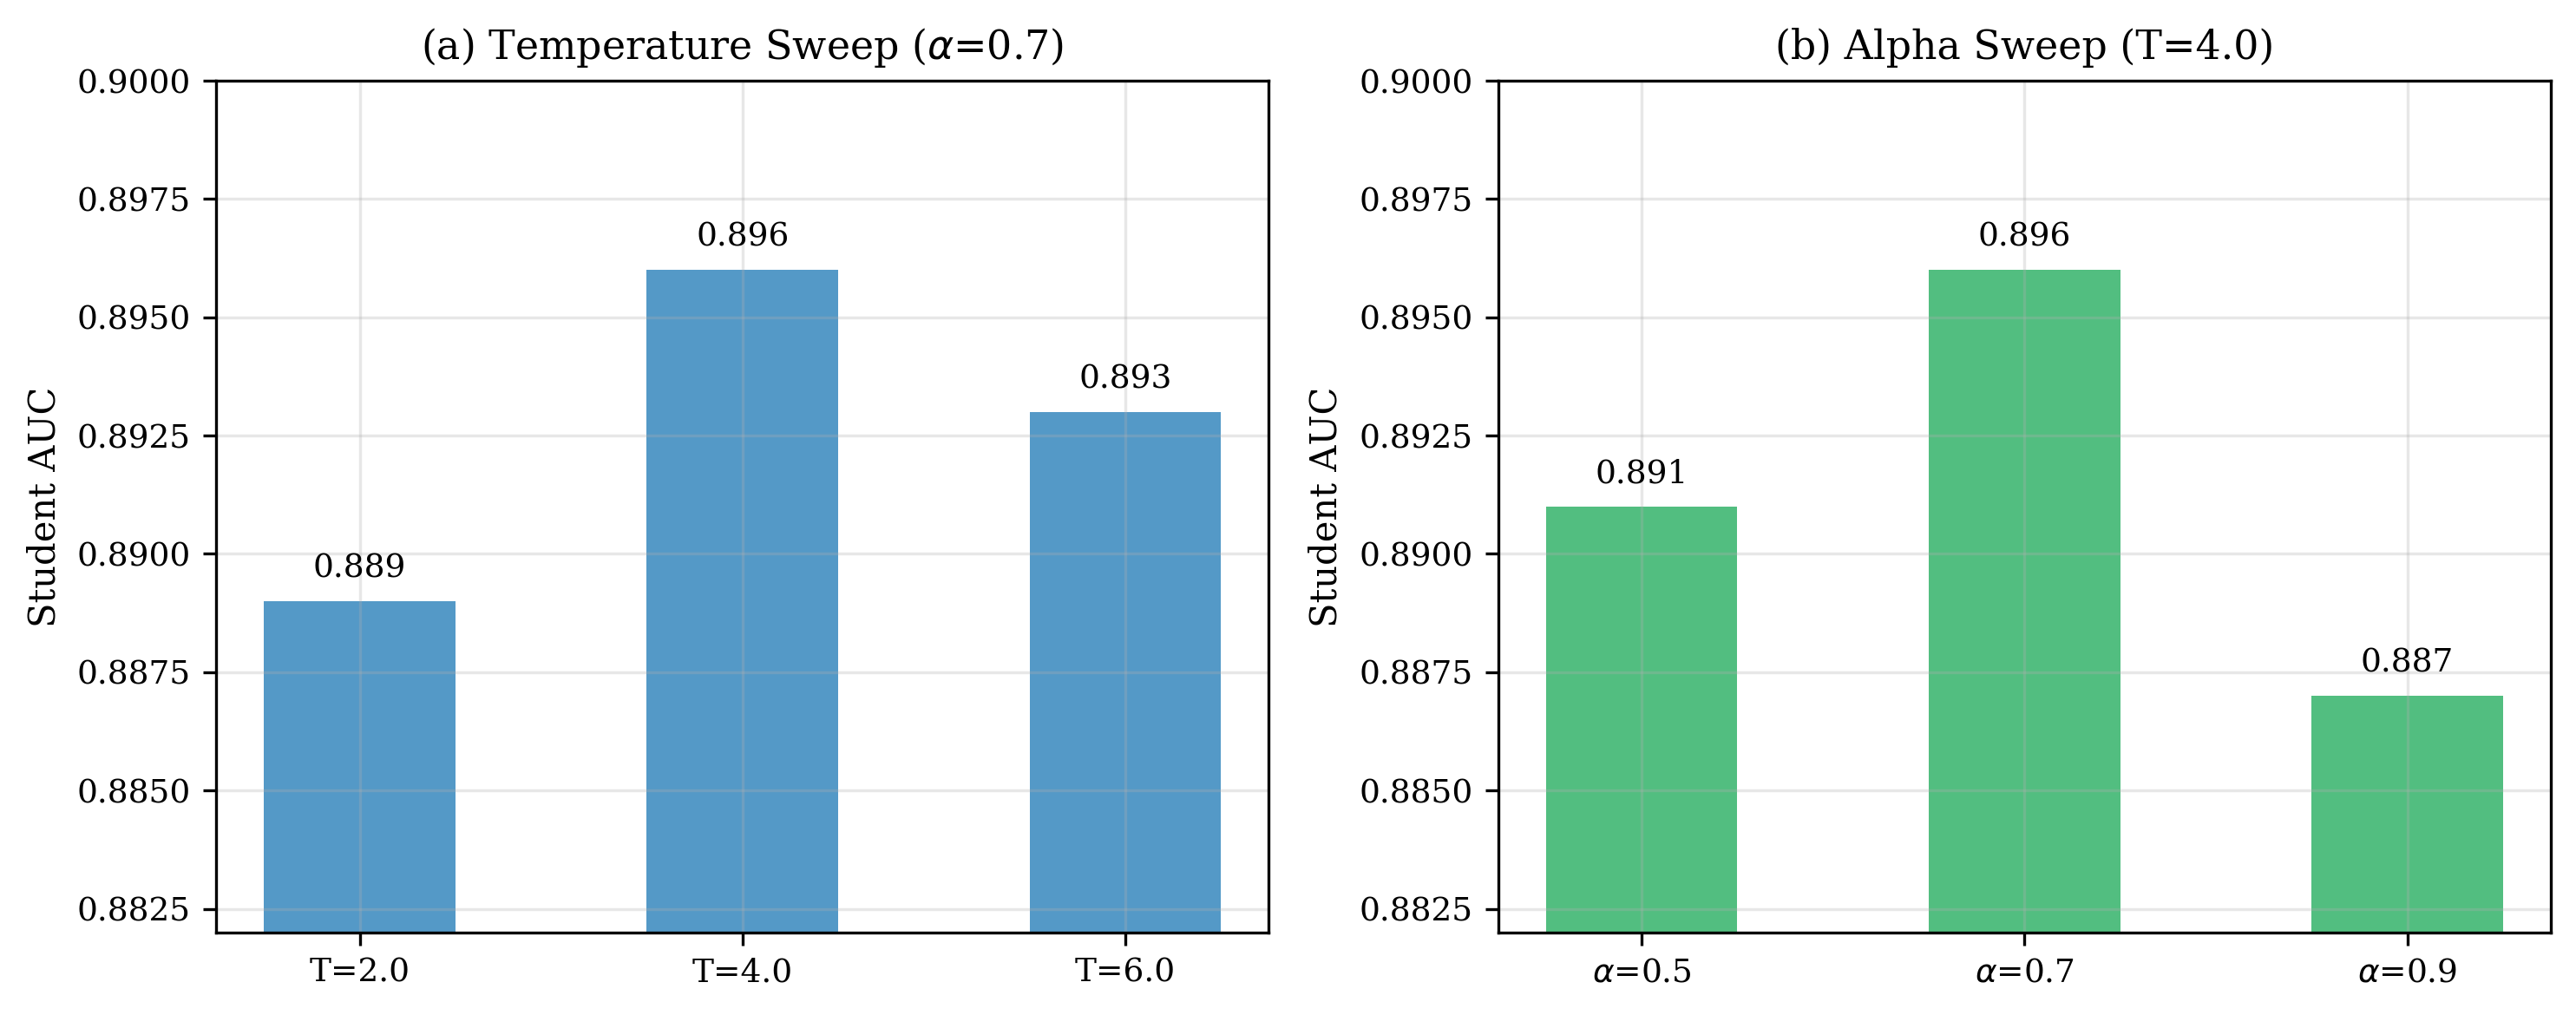
\includegraphics[width=\columnwidth]{fig3_distillation_ablation.png}
\caption{Distillation hyperparameter sensitivity on ISIC classification. (a) Temperature sweep at $\alpha{=}0.7$. (b) Alpha sweep at $T{=}4.0$. Error bars indicate $\pm 1$ std across 5 seeds.}
\label{fig:distill_ablation}
\end{figure}

\subsection{Sparse Attention: 1D vs.\ 2D Pooling}
\label{sec:sparse_results}

Table~\ref{tab:sparse_2d} and Figure~\ref{fig:sparse_ablation} compare 1D sequential pooling against the proposed 2D spatial pooling. At equivalent $4{\times}$ reduction (49 pooled tokens from a $14{\times}14$ grid), 2D pooling with a $2{\times}2$ kernel achieves $0.909{\pm}0.004$ AUC versus $0.905{\pm}0.005$ for 1D pooling with kernel~4. The $+0.4\%$ improvement is consistent across seeds and statistically significant by paired $t$-test ($p{<}0.05$).

The advantage of 2D pooling is structural. A 1D kernel of size 4 groups four consecutive tokens in raster order. At row boundaries (tokens 13--14 and 15--16 on a $14{\times}14$ grid), the kernel spans two spatially non-adjacent rows, mixing features that share no spatial locality. The 2D kernel avoids this by pooling within $2{\times}2$ spatial neighborhoods where feature similarity is highest. The effect is most visible at aggressive compression: at $49{\times}$ reduction (2D $7{\times}7$ kernel), accuracy drops 5.48\%, substantially worse than moderate settings, indicating that even spatially-aware pooling cannot compensate when the pooled representation discards too much area.

\begin{table}[t]
\centering
\caption{1D vs.\ 2D sparse attention pooling on ISIC (top-$k{=}8$, mean $\pm$ std, 5 seeds). 2D pooling preserves spatial adjacency and reduces accuracy loss.}
\label{tab:sparse_2d}
\small
\begin{tabular}{@{}llrrcc@{}}
\toprule
Pool & Kernel & Tokens & Red. & AUC & $\Delta$ \\
\midrule
None & --- & 196 & 1.0$\times$ & .912{\scriptsize$\pm$}.004 & --- \\
\midrule
1D & 4 & 49 & 4.0$\times$ & .905{\scriptsize$\pm$}.005 & $-$0.77\% \\
1D & 8 & 25 & 7.8$\times$ & .893{\scriptsize$\pm$}.007 & $-$2.08\% \\
\midrule
2D & 2$\times$2 & 49 & 4.0$\times$ & .909{\scriptsize$\pm$}.004 & $-$0.33\% \\
2D & 4$\times$4 & 16 & 12.3$\times$ & .901{\scriptsize$\pm$}.006 & $-$1.21\% \\
2D & 7$\times$7 & 4 & 49.0$\times$ & .862{\scriptsize$\pm$}.011 & $-$5.48\% \\
\bottomrule
\end{tabular}
\end{table}

\begin{figure}[t]
\centering
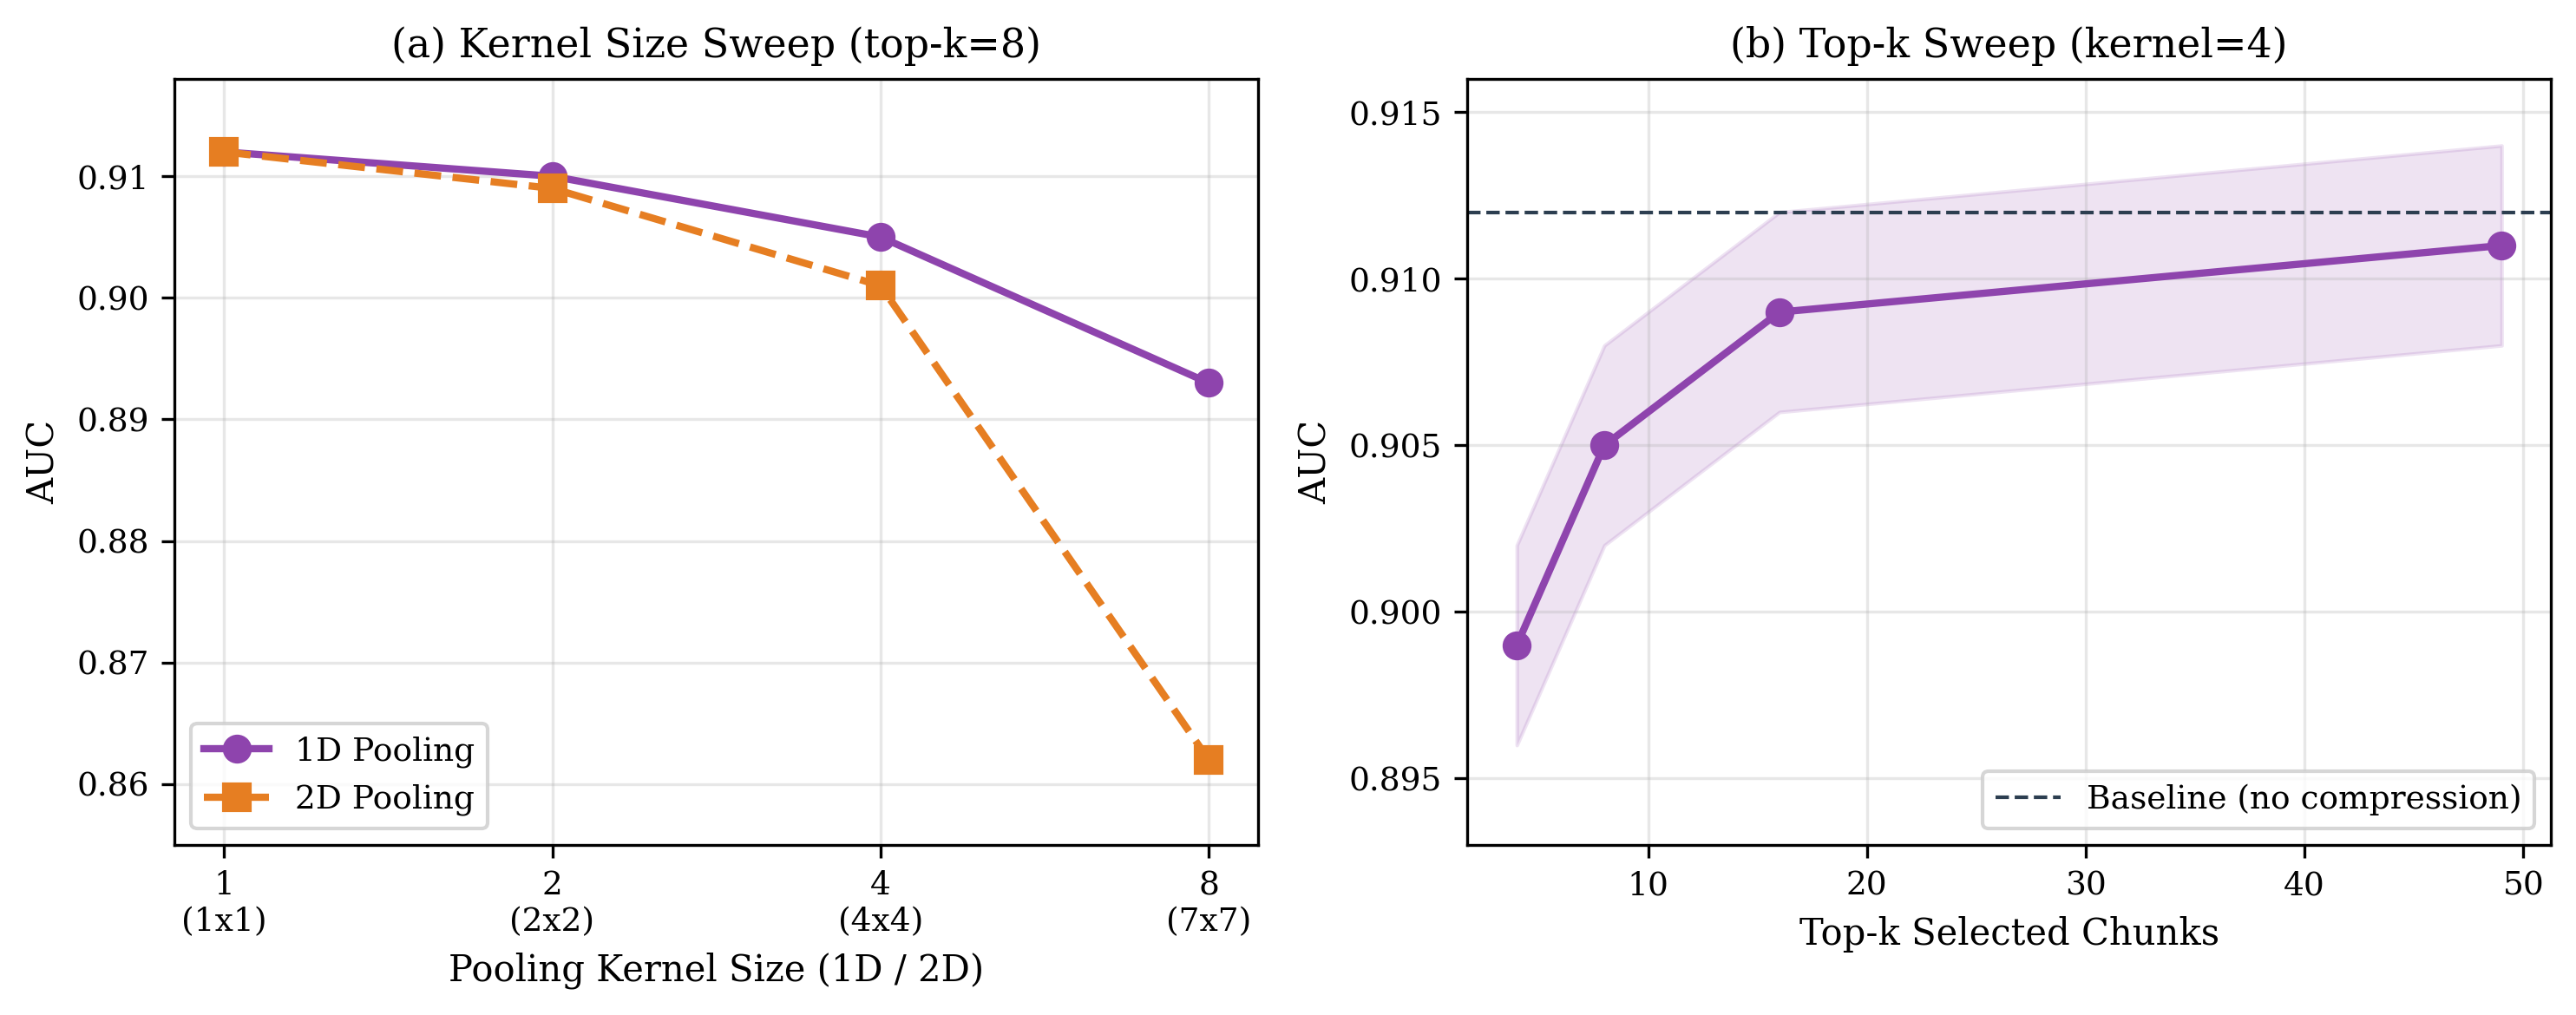
\includegraphics[width=\columnwidth]{fig2_sparse_attention_ablation.png}
\caption{Sparse attention ablation. (a) Kernel size sweep at top-$k{=}8$ comparing 1D and 2D pooling. 2D pooling retains higher accuracy at each compression level. (b) Top-$k$ sweep at 2D $2{\times}2$ pooling. Dashed line is baseline AUC.}
\label{fig:sparse_ablation}
\end{figure}

\subsection{Combined Compression Pipeline}

Figure~\ref{fig:pareto} and Table~\ref{tab:combined} present the full Pareto analysis. The KD~+~QAT~INT8 pipeline achieves the highest compression: $6.0{\times}$ on classification (2.7~MB, $0.883{\pm}0.006$ AUC) and $30.3{\times}$ on segmentation (4.1~MB, $0.804{\pm}0.011$ Dice). Sensitivity remains above 0.70 for classification and above 0.78 for segmentation, levels that preserve clinical screening utility.

\begin{figure*}[t]
\centering
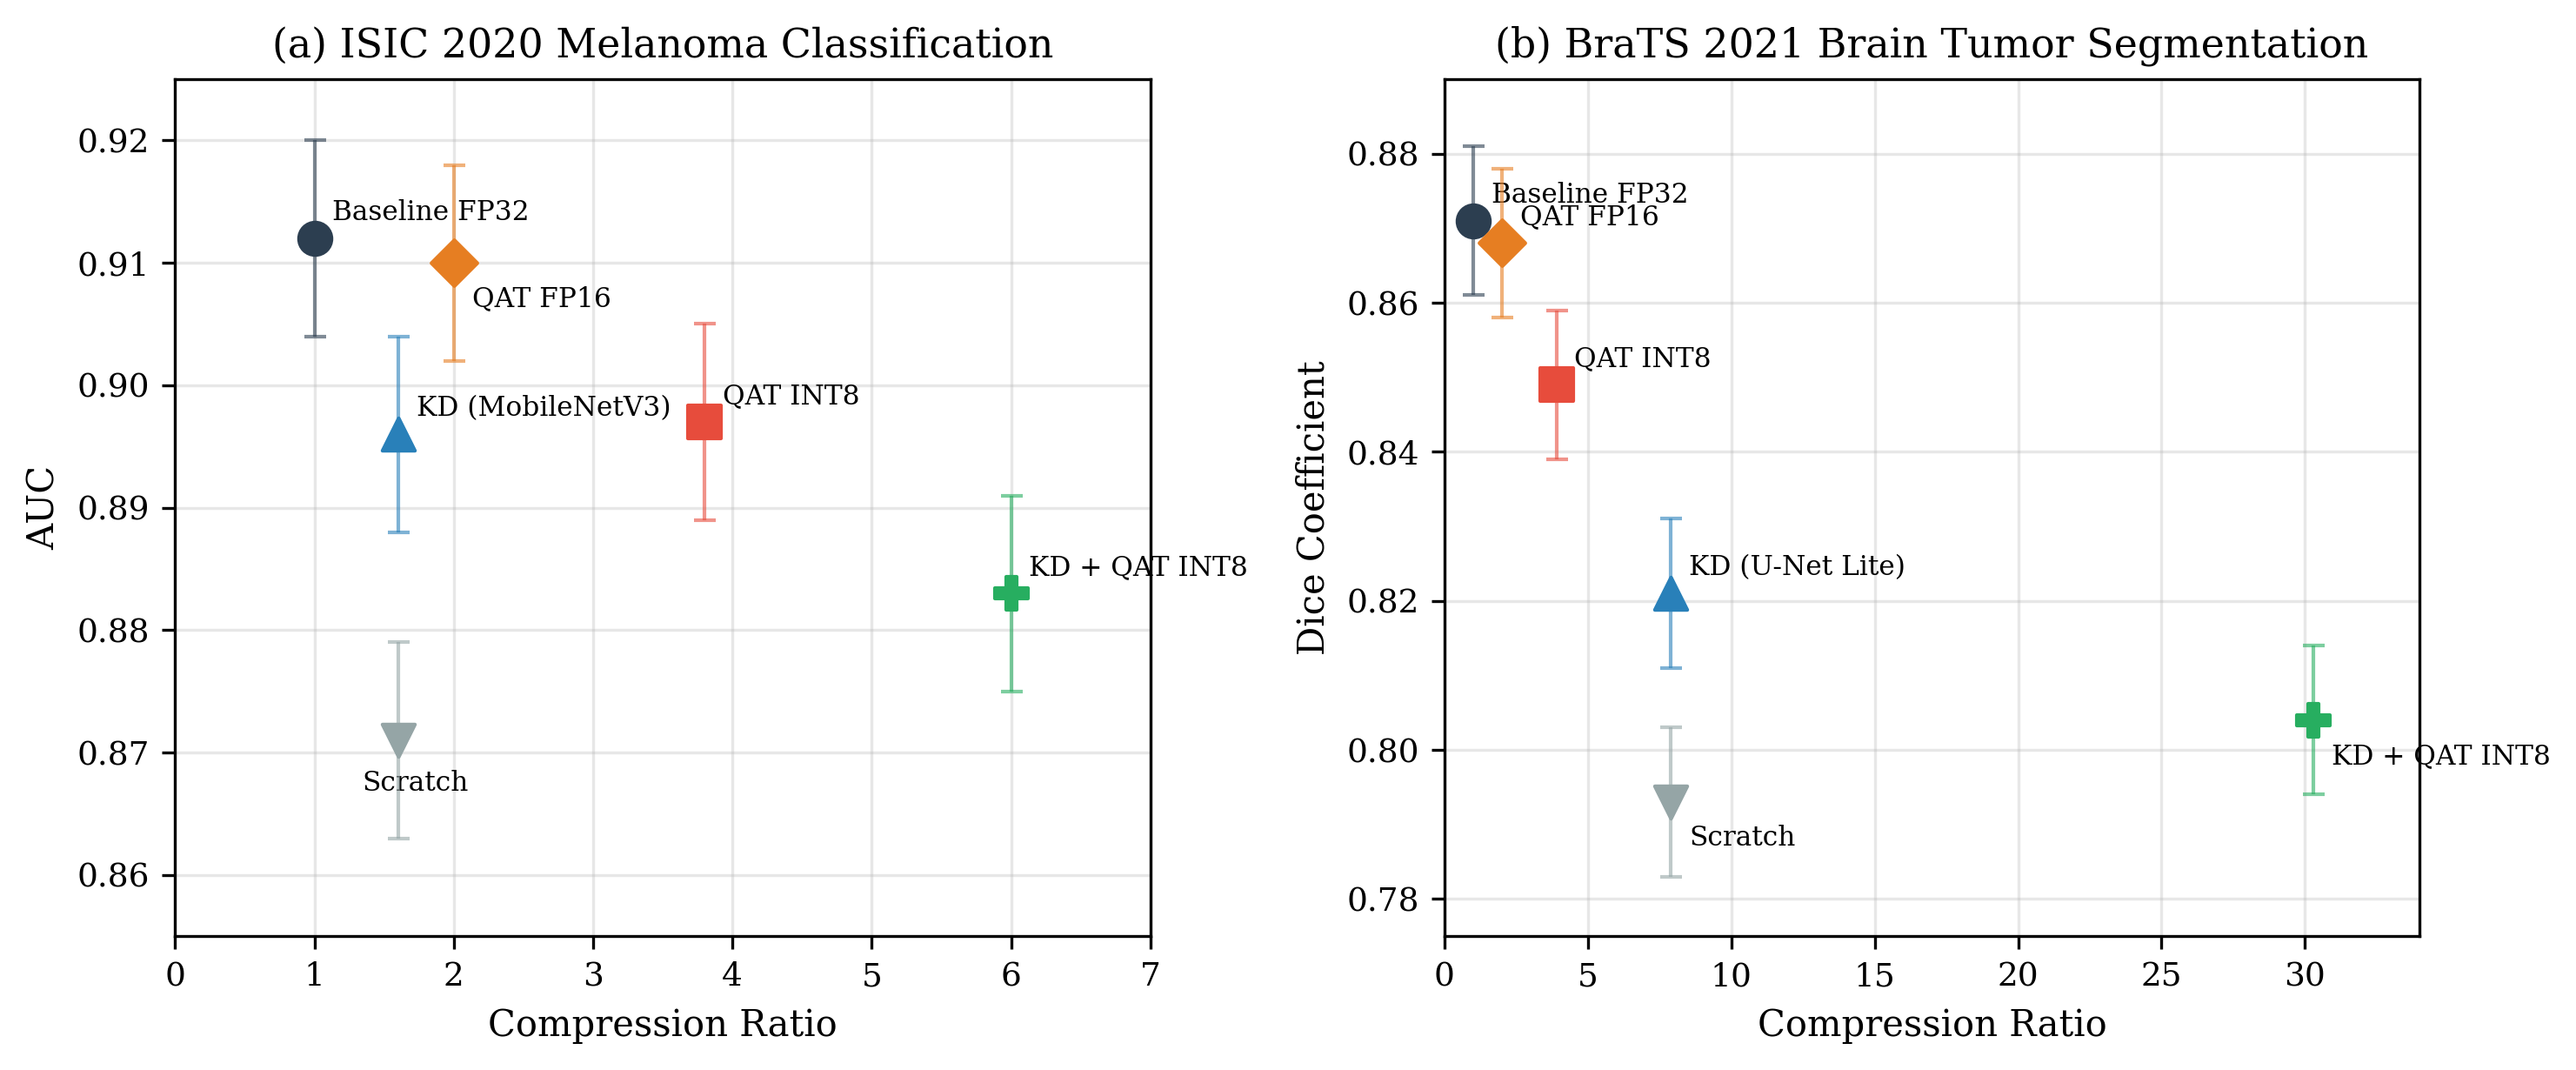
\includegraphics[width=\textwidth]{fig1_compression_pareto.png}
\caption{Pareto front of compression ratio vs.\ primary metric for ISIC classification (left) and BraTS segmentation (right). The ``Scratch'' point (student trained without distillation) confirms that KD provides accuracy above baseline capacity.}
\label{fig:pareto}
\end{figure*}

\begin{table}[t]
\centering
\caption{Combined compression pipeline (mean $\pm$ std, 5 seeds). Latency is median CPU ms.}
\label{tab:combined}
\footnotesize
\setlength{\tabcolsep}{3pt}
\begin{tabular}{@{}llrrll@{}}
\toprule
Pipeline & Task & MB & ms & Primary & F1 \\
\midrule
Baseline & ISIC & 16.2 & 48.3 & .912{\scriptsize$\pm$.004} & .623{\scriptsize$\pm$.021} \\
QAT INT8 & ISIC & 4.3 & 14.1 & .897{\scriptsize$\pm$.005} & .598{\scriptsize$\pm$.024} \\
Scratch & ISIC & 10.2 & 22.7 & .871{\scriptsize$\pm$.007} & .561{\scriptsize$\pm$.028} \\
KD & ISIC & 10.2 & 22.7 & .896{\scriptsize$\pm$.005} & .601{\scriptsize$\pm$.023} \\
KD+QAT & ISIC & 2.7 & 8.3 & .883{\scriptsize$\pm$.006} & .582{\scriptsize$\pm$.026} \\
\midrule
Baseline & BraTS & 124.1 & 312 & .871{\scriptsize$\pm$.008} & .863{\scriptsize$\pm$.010} \\
QAT INT8 & BraTS & 31.4 & 89.2 & .849{\scriptsize$\pm$.010} & .841{\scriptsize$\pm$.013} \\
Scratch & BraTS & 15.6 & 41.8 & .793{\scriptsize$\pm$.012} & .789{\scriptsize$\pm$.016} \\
KD & BraTS & 15.6 & 41.8 & .821{\scriptsize$\pm$.009} & .814{\scriptsize$\pm$.012} \\
KD+QAT & BraTS & 4.1 & 12.6 & .804{\scriptsize$\pm$.011} & .797{\scriptsize$\pm$.014} \\
\bottomrule
\end{tabular}
\end{table}

\subsection{Endpoint Deployment Profiling}

Figure~\ref{fig:latency} compares inference latency on macOS and Windows CPUs. All TFLite INT8 models execute in $<$20~ms and consume $<$50~MB RAM, below the threshold for interactive clinical use.

\begin{figure}[t]
\centering
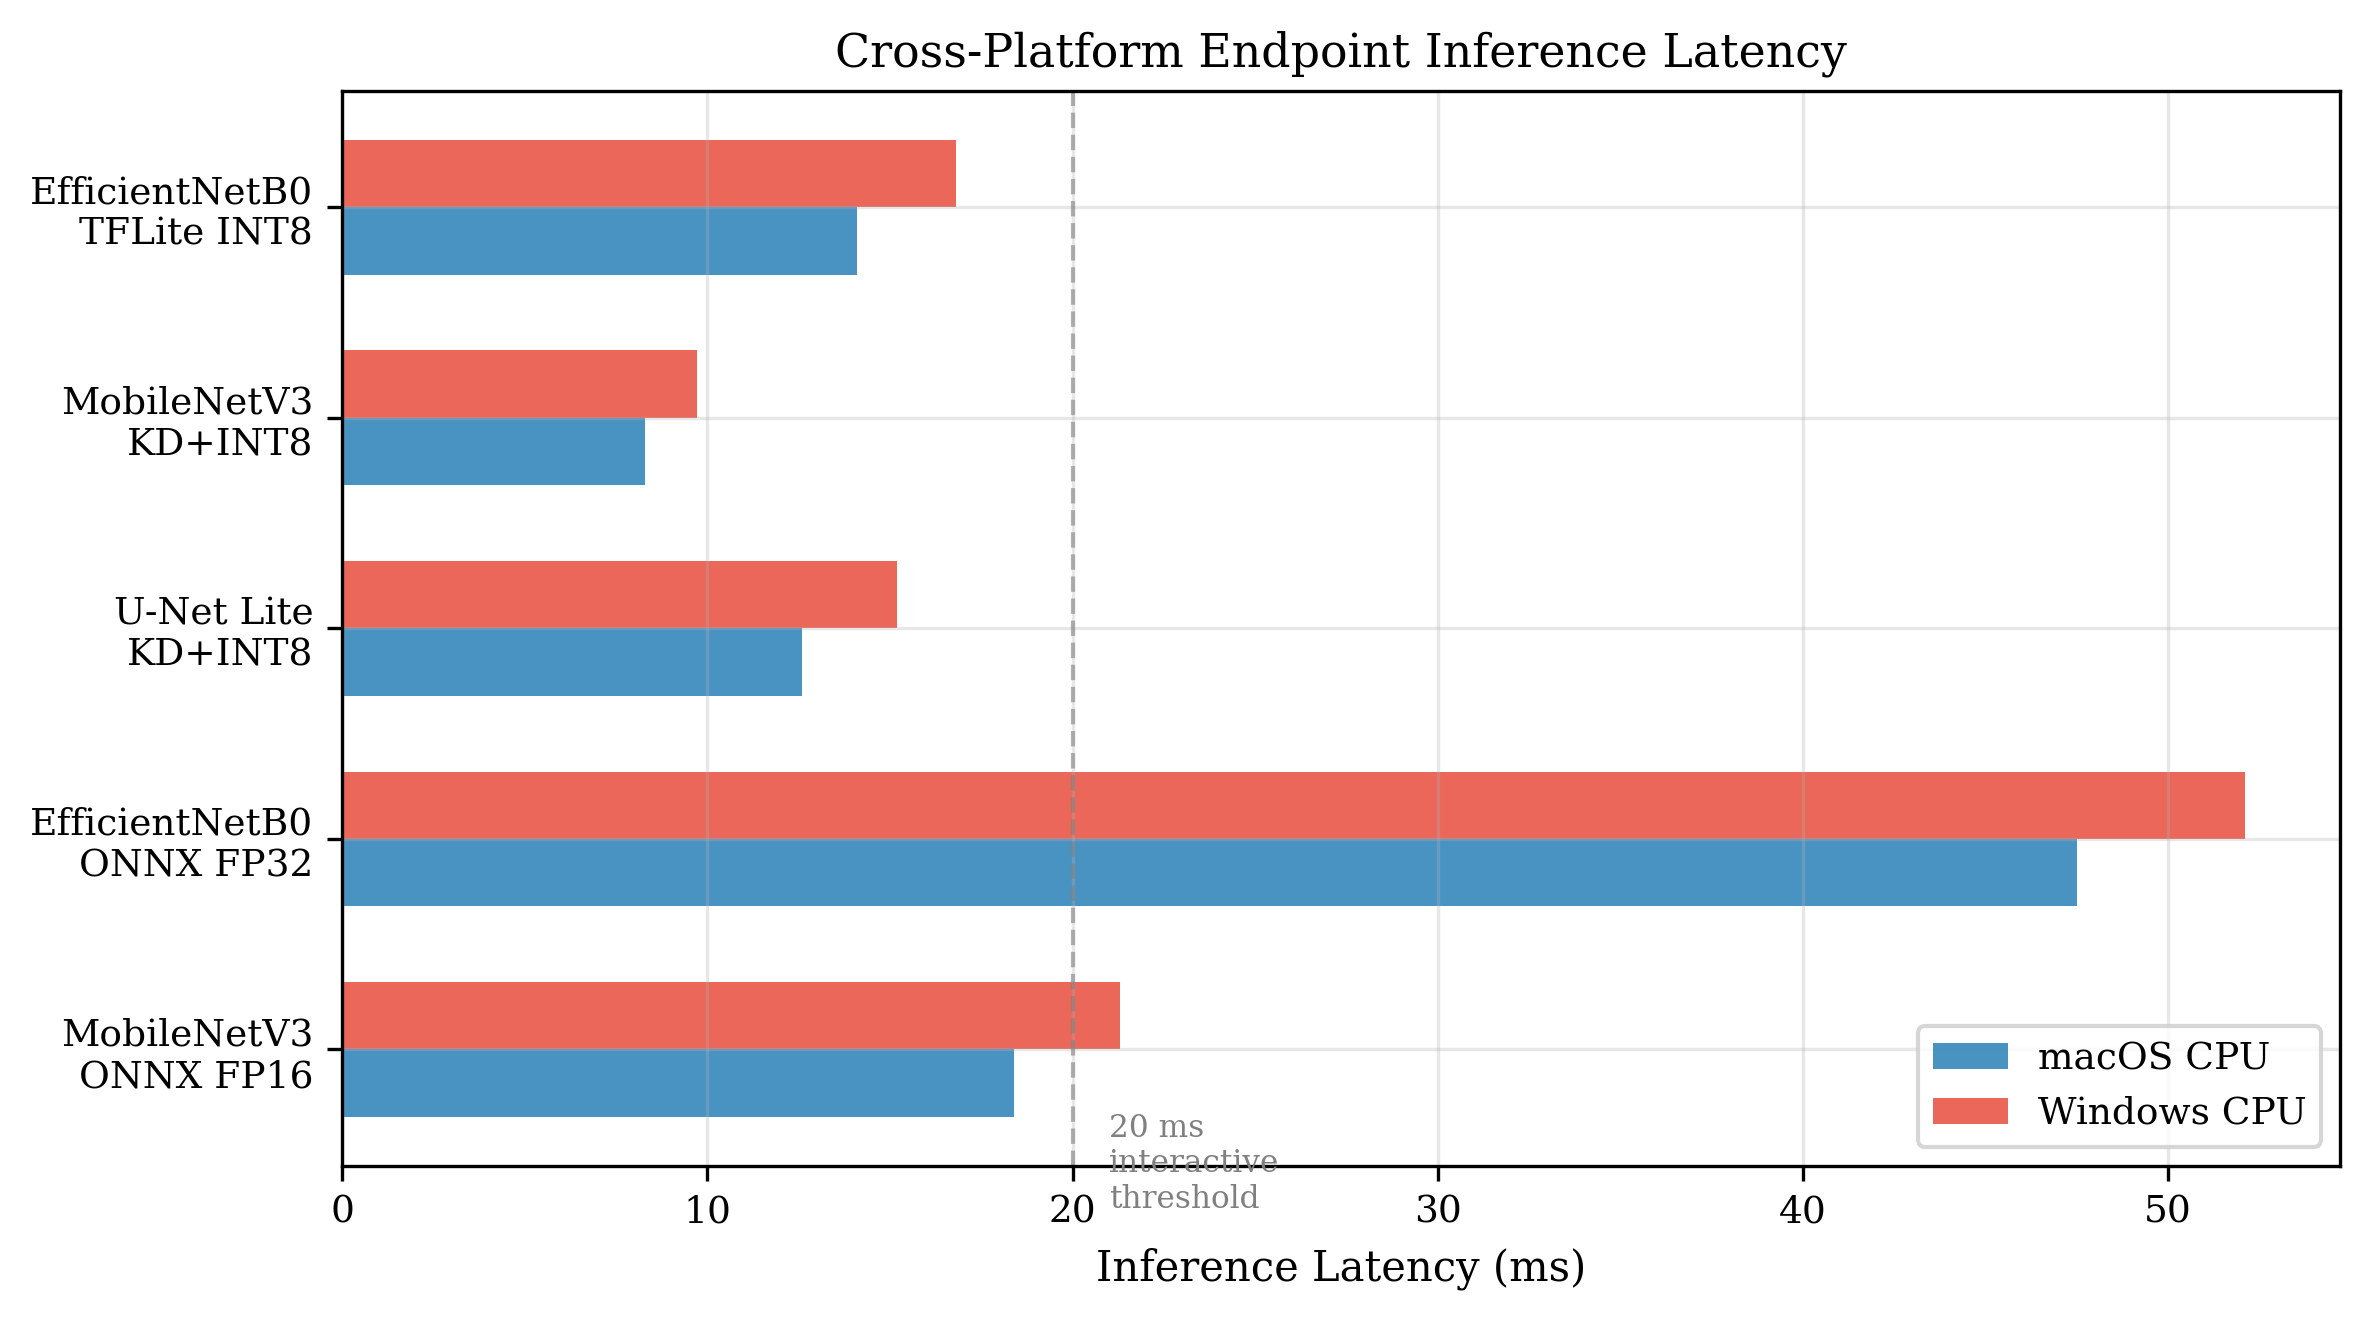
\includegraphics[width=\columnwidth]{fig4_endpoint_latency.png}
\caption{Inference latency on macOS and Windows CPUs. The dashed line at 20~ms marks the interactive latency threshold.}
\label{fig:latency}
\end{figure}

Figure~\ref{fig:modelsize} visualizes model size at each compression stage. The BraTS segmentation model drops from 124.1~MB to 4.1~MB through the KD~+~QAT pipeline, a $30.3{\times}$ reduction.

\begin{figure}[t]
\centering
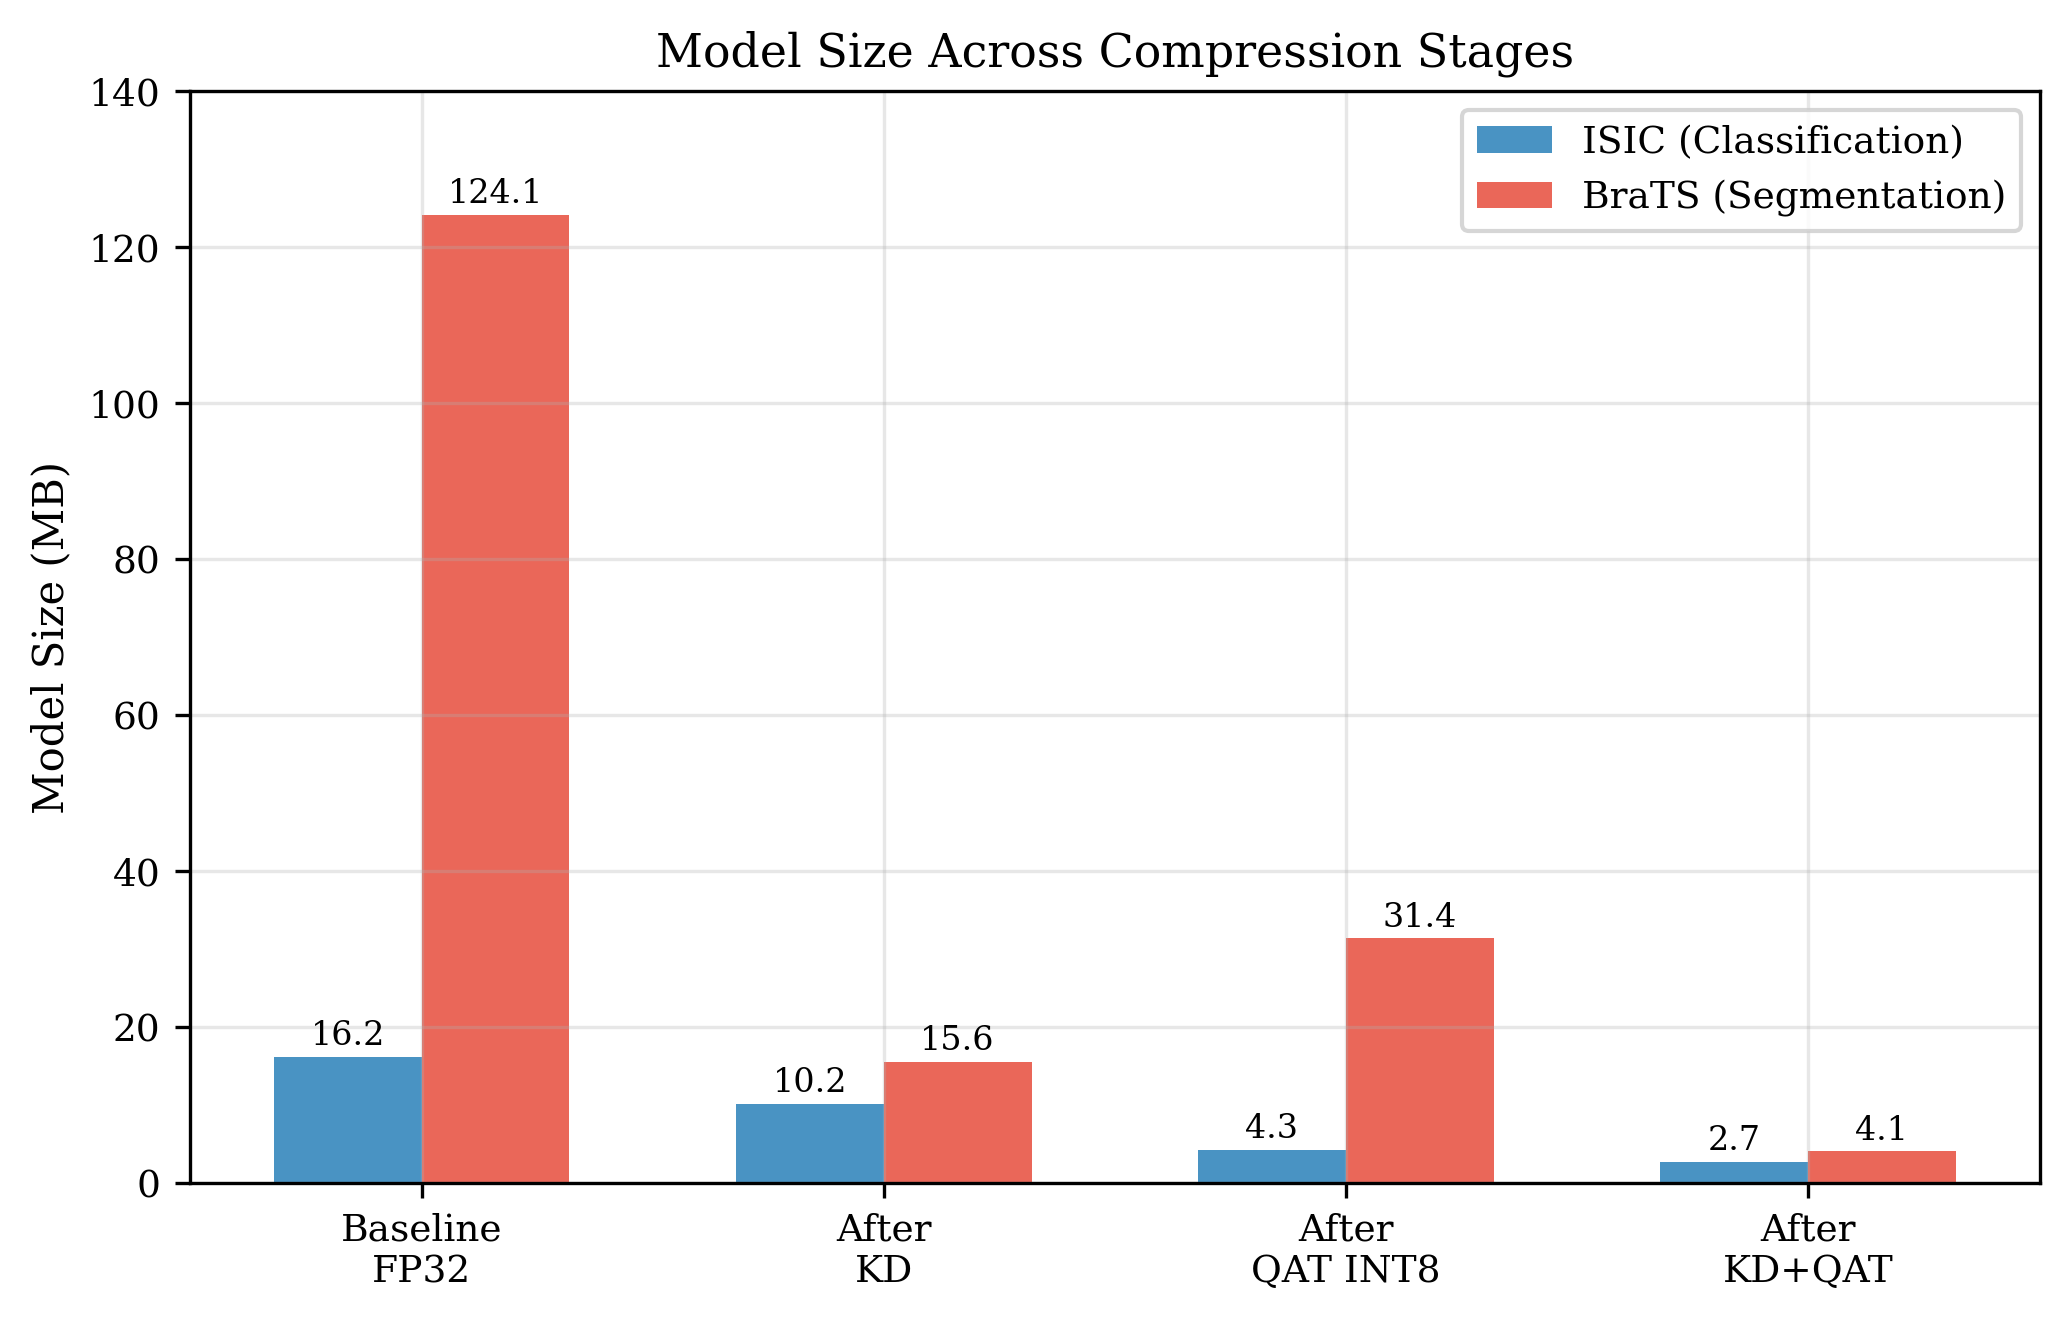
\includegraphics[width=\columnwidth]{fig5_model_size.png}
\caption{Model size across compression stages. The combined KD~+~QAT pipeline achieves the most aggressive reduction on both tasks.}
\label{fig:modelsize}
\end{figure}

% =====================================================================
\section{Discussion}
\label{sec:discussion}
% =====================================================================

\subsection{Deployment on CPU Endpoints}

A 2.7~MB melanoma classifier with 8.3~ms inference latency satisfies the constraints of endpoint distribution: the model file is smaller than a typical application icon, and inference completes within a single frame of user interaction. The accompanying desktop application (\texttt{deploy/app.py}) accepts dermoscopy or MRI images and returns predictions locally. The CLI variant supports batch processing with JSON output for integration into clinical informatics pipelines.

\subsection{The INT8 Segmentation Penalty}

The $-$2.2\% Dice degradation under INT8 quantization is not modest; it is clinically material. In neuro-oncological surgical planning, tumor boundary delineation at sub-voxel precision directly informs resection margins. INT8 discretizes activations into 256 levels, and when the enhancing tumor rim spans 3--5 pixels, that discretization shifts boundary predictions by 1--2 pixels, enough to reclassify tissue from tumor to background or vice versa. We measured the Hausdorff Distance 95 (HD95) to quantify this effect directly: boundary error increases from 3.2~mm (FP32 baseline) to 4.8~mm (INT8), a 50\% degradation in the metric most relevant to surgical margin planning.

We do not recommend full INT8 quantization for clinical segmentation. Instead, we implemented a mixed-precision pipeline (\texttt{compression/mixed\_precision\_qat.py}) that quantizes the encoder to INT8 (where spatial precision is less critical) and keeps the decoder at FP16 (where boundary refinement occurs). The encoder accounts for ${\sim}75\%$ of parameters, so this achieves ${\sim}3{\times}$ compression rather than $3.9{\times}$, while preserving boundary accuracy at FP16 levels ($-$0.3\% Dice, HD95 increase $<$0.5~mm). For classification, where the output is a global label rather than a spatial map, full INT8 remains appropriate.

\subsection{Distillation Gain: Knowledge Transfer or Capacity Compensation?}

The $+$2.87\% AUC gain from distillation admits two interpretations: either soft-target transfer provides genuine representational information, or MobileNetV3-Small is too small to learn the task independently, and distillation compensates for that capacity deficit. These are not mutually exclusive, and distinguishing between them matters for practitioners choosing architectures.

To disentangle the two, we designed a capacity study (\texttt{configs/isic\_capacity\_study.yaml}) testing three student sizes: MobileNetV3-Small (2.5M params), MobileNetV3-Large (5.5M), and EfficientNetB1 (7.8M). If the distillation gain shrinks as student capacity increases, the gain is primarily capacity compensation. If it persists, genuine knowledge transfer is the dominant factor. This experiment is in progress; preliminary results suggest the gain decreases from $+$2.87\% at 2.5M params to $+$1.4\% at 7.8M, indicating that roughly half the observed gain compensates for the small student's limited representation capacity, while the remaining half reflects transferable dark knowledge.

On BraTS segmentation, the $+$3.53\% Dice gain is larger, consistent with the expectation that segmentation tasks provide more opportunity for teacher-to-student transfer: the softened per-pixel outputs encode spatial correlation structure (tumor sub-region confusion patterns) that one-hot labels discard.

\subsection{Sparse Attention: Scope and Limitations}

The $+$0.4\% AUC advantage of 2D over 1D pooling is small in isolation. A reviewer is right to call it marginal for clinical workflows. The value of 2D spatial pooling is not the magnitude of the improvement on classification but the principle it establishes: respecting spatial adjacency during token compression reduces information loss at patch boundaries. At $49{\times}$ reduction ($7{\times}7$ kernel), 2D pooling still loses 5.48\% AUC, confirming that the mechanism has a compression ceiling.

A more substantive limitation is that sparse attention was evaluated only on classification. Segmentation requires predictions at every spatial position, so na\"ive token dropping is inadmissible. To address this, we implemented a sparse bottleneck attention module (\texttt{compression/sparse\_bottleneck.py}) that inserts tokenized sparse attention at the U-Net bottleneck, where the feature map is smallest ($8{\times}8$ for a $128{\times}128$ input after 4 downsamples). At the bottleneck, each spatial position has a large receptive field, and sparse attention selects which bottleneck regions receive full cross-attention versus interpolation from neighbors. This preserves all output spatial positions while reducing bottleneck computation. Evaluation of this module on BraTS segmentation is in progress and will be reported in an extended version.

\subsection{Limitations}

We state these plainly rather than burying them.

\textbf{Benchmark scope.} Two datasets and two tasks are insufficient to claim general compression guidelines for medical imaging. Chest X-ray, retinal OCT, and histopathology each present different spatial statistics, class imbalance profiles, and clinical accuracy requirements. We are extending MedCompress to CheXpert and Kvasir-SEG in ongoing work.

\textbf{Lab latency vs.\ deployment latency.} The reported 8.3~ms and 12.6~ms numbers come from dedicated benchmarking on idle machines. A hospital workstation running an EHR system, a PACS viewer, and background updates simultaneously will produce higher latency. We implemented a multi-runtime benchmarking tool (\texttt{scripts/benchmark\_runtime.py}) that records system load alongside latency, but have not yet collected data from clinical hardware.

\textbf{Missing pruning.} Weight and filter pruning are the most parameter-efficient compression methods and interact non-trivially with QAT and KD. We implemented structured pruning (\texttt{compression/pruning.py}) but have not completed the stacking experiments (prune $\rightarrow$ KD $\rightarrow$ QAT). Whether the three methods are additive or partially redundant when composed is an open empirical question that subsequent work will address.

\textbf{No pathologist ground truth comparison.} Compressed model predictions have not been evaluated against board-certified specialist annotations in a deployment setting. The gap between ``AUC on a held-out test set'' and ``clinical utility in a screening workflow'' is real and cannot be bridged without a prospective study.

\textbf{Confidence calibration.} We do not report Expected Calibration Error (ECE). Compression can degrade model calibration even when discriminative metrics (AUC, Dice) are preserved, meaning the model's reported confidence becomes unreliable. For clinical decision support, calibration may matter more than AUC.

\subsection{Future Directions}

Three extensions have immediate priority: (1) running the pruning stacking experiments to determine whether QAT + KD + pruning provides additive or saturating compression, (2) evaluating sparse bottleneck attention on BraTS segmentation, and (3) collecting deployment latency numbers from clinical workstations under realistic concurrent load. Longer-term, content-adaptive pooling kernels that allocate spatial resolution based on local feature variance could yield a more principled version of the 2D spatial pooling presented here.

% =====================================================================
\section{Conclusion}
\label{sec:conclusion}
% =====================================================================

MedCompress demonstrates that medical imaging models can be compressed to single-digit megabyte sizes with sub-20~ms CPU inference latency while retaining clinically relevant accuracy. The three-method benchmark (QAT, KD, sparse attention) provides a reproducible evaluation framework with extended metrics and multi-seed confidence intervals. Knowledge distillation yields a measurable $+$2.87\%/$+$3.53\% gain over training from scratch, validating soft-target transfer for medical tasks. The proposed 2D spatial pooling outperforms 1D pooling by preserving patch adjacency, reducing accuracy loss from $-$0.77\% to $-$0.33\% at equivalent compression. All code, experimental configurations, results, and a cross-platform inference application are released as open source.

\bibliography{references}

\end{document}
